\documentclass[conference]{IEEEtran}
\IEEEoverridecommandlockouts
% The preceding line is only needed to identify funding in the first footnote. If that is unneeded, please comment it out.
\usepackage{cite}
\usepackage{amsmath,amssymb,amsfonts}
\usepackage{algorithmic}
\usepackage{graphicx}
\usepackage{textcomp}
\usepackage{xcolor}
\def\BibTeX{{\rm B\kern-.05em{\sc i\kern-.025em b}\kern-.08em
    T\kern-.1667em\lower.7ex\hbox{E}\kern-.125emX}}
\begin{document}

\title{HyperMI: A Privilege-level Secure Execution Environment for VM Protection against Compromised Hypervisor}
%1\textsuperscript{st}
\author{\IEEEauthorblockN{Wenqing Liu,Kunli Lin,Kun Zhang,Bibo Tu}
\IEEEauthorblockA{\textit{Institute of Information Engineering, Chinese Academy of Sciences} \\
\textit{School of Cyber Security, University of Chinese Academy of Sciences}\\
%\{xxx\}@iie.ac.cn}%
\{liuwenqing,linkunli,zhangkun,tubibo\}@iie.ac.cn}


}

\maketitle

\begin{abstract}

\iffalse
Underlying hypervisor provides all kinds of services for VMs including resource allocation, resource management and so on. Sensitive data and critical content in guest virtual machine is easy to be leaked once hypervisor is compromised. 
%For example, VM escape attack that attackers escape from a guest VM and attack directly the hypervisor. 
%And 
Cross-domain attack is that a malicious VM attacks another VM who shares the same hypervisor once the hypervisor is attacked. Therefore, VM isolation is important to protect the memory of VM from compromised hypervisor's malicious access causally. Previous efforts employ extra customized hardware which is not convenient for cloud providers to adopt widely. Or they employ new architecture relying on a higher privilege level which introduces high performance overhead.

%(Hypervisor monitor and isolation)
This paper proposes HyperMI, a novel approach that provides a privilege-level secure execution environment  for VM isolation protection in cloud computing against compromised hypervisor. In order to achieve the goal that it can prevent customers' sensitive data in VM from being leaked once the hypervisor is attacked.
%It provides a privilege-level secure isolated execution environment as TCB, named HyperMI world. This world is used for effective VM isolation and event-driven VM monitoring.
It provides HyperMI world, effective VM isolation and event-driven VM monitoring. HyperMI world is a privilege-level secure isolated execution environment as TCB, and the world is used for VM isolation and VM monitoring.
%Unlike other approaches of protecting VM, 
Instead of being placed at a higher level,
HyperMI world is placed at the same privilege level with the compromised hypervisor, incurring low overhead. Effective VM isolation provides the runtime protection for VM by using a novel way that isolate memory among VMs and hypervisor securely. 
%The event-driven VM monitoring can ensure the accuracy which polling-inquire can't provide. 
The event-driven VM monitoring can ensure the secure interaction between VM and hypervisor.
%The key of
What's the most important, HyperMI focuses on decoupling the function of monitoring interaction between hypervisor and VM into VM monitoring module and decoupling the function of memory isolation from hypervisor into VM isolation module. As a result, HyperMI controls page mapping, page accessing and isolates memory completely when page is allocated to VM.
We have implemented a prototype for KVM hypervisor with multiple Linux as guest OSes, which can be used in commercial cloud computing industry with portability and compatibility for all kinds of CPU platforms. The security analysis shows that this approach can provide protection for VM with effective isolation and event-driven monitoring, and the performance evaluation confirms the efficiency of HyperMI.

Sensitive data in guest virtual machine is easy to be leaked once hypervisor is compromised.
Therefore, VM protection is important to protect the memory of VM from compromised hypervisor’s malicious access causally. Previous efforts employ extra customized hardware or employ new software relying on a higher privilege level than hypervisor.

This paper proposes HyperMI, a novel approach that provides a privilege-level secure execution environment for VM protection in cloud computing against compromised hypervisor. 
It provides HyperMI world, effective VM isolation and event-driven VM monitoring in order to prevent customers' sensitive data in VM from being leaked.
HyperMI world, placed at the same privilege level with hypervisor, is a privilege-level secure isolated execution environment. As TCB, it is used for VM isolation and VM monitoring. 
What's the most important, HyperMI focuses on decoupling the function of interaction between hypervisor and VM and decoupling the function of address mapping of VM from hypervisor.
As a result, HyperMI can only controls page mapping of VM and EPT updating when a page is allocated to a VM.
We have implemented a prototype for KVM hypervisor with multiple Linux as guest OSes, which can be used in commercial
cloud computing industry with portability and compatibility for all kinds of CPU platforms. The security analysis shows that this approach can provide protection for VM with effective isolation and event-driven monitoring, and the performance evaluation confirms the efficiency of HyperMI.
\fi
Once compromising the hypervisor, remote or local adversaries can easily access other customers’ sensitive data in the memory and context of guest virtual machines (VMs).
%VM is easy to be subveted once the hypervisor is compromised. 
% Therefore, VM protection is important to protect the memory of VM from compromised hypervisor's malicious access causally. Previous efforts employ extra customized hardware or employ new software relying on a higher privilege level than hypervisor.
Therefore, it is important to protect VM, especially the context and the memory of VM from compromised hypervisor.
\iffalse
However, previous efforts employ extra customized hardware which is not convenient for cloud providers to adopt widely. Or they employ new architecture relying on a higher privilege level which introduces high performance overhead. 
\fi

This paper proposes HyperMI, a novel approach to supply VM runtime protection based on a privilege-level secure execution environment in cloud computing against compromised hypervisor. 
Firstly, we propose HyperMI world which is a secure and isolated trusted execution environment. HyperMI world is designed to be placed at the same privilege-level with hypervisor and does not rely on any additional hardware or a higher privileged level than hypervisor. Secondly, we propose event-driven VM monitoring which intercepts interaction between all VMs and hypervisor, and redirect interaction process to HyperMI for VM protection. Thirdly, we propose effective VM isolation to provide runtime protection for VM by isolating memory among VMs and hypervisor securely. 
The key of HyperMI is that HyperMI decouples the functions of interaction between VMs and hypervisor, and the functions of address mapping of VM from the compromised hypervisor. As a result, HyperMI isolates memory completely, controls memory mapping when a page is allocated to VM, and resists malicious memory of VM accessing from compromised hypervisor.
We have implemented a prototype for KVM hypervisor with multiple Linux as guest OSes, which can be used in commercial cloud computing industry with portability and compatibility for all kinds of CPU platforms. The security analysis shows that this approach can provide protection for VM with effective isolation and event-driven monitoring, and the performance evaluation confirms the efficiency of HyperMI.




\end{abstract}

\begin{IEEEkeywords}
Virtualization, VM Isolation, VM Security
\end{IEEEkeywords}

\section{Introduction}



As more and more functionalities are added into hypervisor, the code bases of commodity hypervisors (KVM or Xen) have been increased to be massive lines. However, recent survey shows that commodity hypervisor incurs more vulnerabilities because of the larger code bases. 
On the one hand, from 2004 to now, there are 130 vulnerabilities about KVM.
%\cite{kvmcve}
Some of them (e.g., CVE-2018-1087)
%\cite{cve2018}
shows high-risk vulnerabilities that can lead to privilege raising behavior and comprehensive compromised hypervisor.
On the other hand, because hypervisor possess the highest privilege in the cloud environment, an attacker who 
%the larger code bases incurs more vulnerabilities which could be exploited by attackers. Since hypervisor is granted with the highest privilege, attackers who 
compromises hypervisor could harm the whole cloud infrastructure and endanger data and computation in the cloud. For example, an attacker can deploy a complete malicious guest VM on the virtualized platform, conducts attacks to the hypervisor and further attack other VMs even the entire platform through illegal data accessing and so on. Some attacks also directly compromise hypervisor.
% with flaw, then attack VMs.
%What's more, trying to detect malicious actions among frequent cloud management operations is similar to looking for a needle in a haystack.
In order to settle down all these threats, some try to detect malicious actions among frequent cloud management operations, but this kind of approach is much similar to that of looking for a needle in a haystack. Therefore, VM isolation and VM monitoring could provide a superior solution from another perspective. 
% To avoid the threats from compromised hypervisor, trying to detect malicious actions among frequent cloud management operations is similar to looking for a needle in a haystack, the most important thing to be considered should be VM isolation and VM monitoring.
%Previous researches
%\cite{Garfinkel2003A,Jiang2007Stealthy,Litty2008Hypervisor,Rhee2009Defeating,Jones2006Antfarm,Kourai2005HyperSpector,Seshadri2007SecVisor}, %use virtualization idea to provide the required secure isolated environment for security tools that monitor and protect the %kernel. We introduce three approaches, customized hardware, reconstructed hypervisor and software at higher privilege level %to provide these service.
Current researches, including customized hardware, reconstructed hypervisor and software placed at a higher privilege level, provide services of protection for critical data.

\textbf{Customized Hardware }
Some efforts (SecureME\cite{Chhabra2011SecureME}, Bastion\cite{Champagne2010Scalable} and Iso-x\cite{Evtyushkin2015Iso}) rely on 
% SecureME\cite{Chhabra2011SecureME}, Bastion\cite{Champagne2010Scalable} and Iso-x\cite{Evtyushkin2015Iso}, these efforts relying on
customized underlying hardware to provide fine-grained protection for VM or in-VM process. 
%SecureME protects an application by using a secure processor substrate from the Operating System (OS) through memory cloaking, permission paging, and system call protection. 
Iso-X provides isolation for security-critical pieces of an application by introducing additional hardware and changes to OS. It controls memory access by introducing ISA instructions. 
Bastion, uses modified microprocessor hardware based on FPGA to protect the storage and runtime memory state of enhanced hypervisor against both software and hardware attacks. So that it provides hardware-protected environment and protection for security-critical OS and application modules in an untrusted software stack. 

%Vigilare\cite{Moon2012Vigilare} and KI-Mon \cite{Lee2013KI} provide monitoring for access operations by introducing extra hardware. 
%Vigilare 
%provides a kernel integrity monitor that is architected to snoop the bus traffic of the host system from a separate independent hardware. It
%adds extra Snooper hardware connections module to the host system for bus snooping. KI-Mon monitors write operation to system bus and monitors %data to write in order to check rootkit attack.
%However, for cloud providers, these approaches means high-cost and low practicality as long as they are carried out widely.
%KI-Mon monitors write operation on system bus and handles data to write in order to check rootkit attack.


%To achieve the goal of VM isolation, some efforts, including NoHype\cite{NoHype} and TrustOSV\cite{TrustOSV}, reconstruct the hypervisor. 
%Both of these approaches introduce lots of modification to the current commodity hypervisor, such as binding the pre-allocated fixed cores and memory %resources to the associated VM. In details, 
% by pre-allocating fixed cores or memory resource.
% to isolate VM via reconstructing hypervisor.
% In the meantime, deprive some virtualization capabilities and introduce lots of modification to hypervisor. And
%NoHype removes the virtualization layer, while retaining the key features enabled by virtualization. TrustOSV provides protection from compromised cloud %environment by removing interaction between exposed executing environment and hypervisor. Another drawback is that these approaches may strip away some %of virtualization capabilities.

\textbf{Reconstructed Hypervisor }
%To achieve the goal of VM isolation, 
Some efforts (NoHype\cite{NoHype} and TrustOSV\cite{TrustOSV}) pre-allocate fixed cores or memory resource to isolate VM via reconstructing hypervisor. In the meantime, deprive some virtualization capabilities and introduce lots of modification to hypervisor. And NoHype removes the virtualization layer, while retaining the key features enabled by virtualization. TrustOSV provides protection from compromised cloud environment by removing interaction between exposed executing environment and hypervisor.

 
\textbf{Software at a Higher Privilege Level}
In order to mitigate the hazard caused by the hypervisor possess at the highest privilege level, plenty of software solutions propose and introduce a higher privilege-level than the original hypervisor. Nested virtualization is one of the representative approaches, who provides a higher-privileged and isolated 
% To protect VMs from compromised hypervisor as possible as we can, more and more software solutions based on a higher privilege level are proposed.
% For example, nested virtualization introduces a higher privilege level and provides an isolated
execution environment to run the monitor securely. The turtles project \cite{Ben2007The} and CloudVisor \cite{Zhang2011CloudVisor} are examples of systems that propose nested virtualization idea to achieve isolation for protected resources. Specially, CloudVisor uses nested virtualization to decouple 
%the security protection from 
resource management into nested hypervisor to provide protection for VM. These approaches based on a higher privilege level than hypervisor would introduce lots of inter privilege level transition, severe performance overhead and a larger code base.
% increase the size of code of nested hypervisor.
%Meanwhile, practicality and low performance overhead are among the most prized features for cloud %providers. For business architectures that are already widely deployed, it is equally important to %minimize changes to existing systems or architectures. However, there is no perfect approach to meet all %the requirements at the same time.

%In summary, for cloud providers, features of system for protecting the security of VMs against compromised hypervisor including low performance %overhead, less modification to system and high practicality are the most important.
Meanwhile, practicality and low performance overhead are among the most prized features for cloud providers. For business architectures that are already widely deployed, it is equally important to minimize changes to existing systems or architectures. Current works can't satisfy all features simultaneously. To avoid introducing extra hardware device and address the high performance overhead of inter-privilege transition for software at a higher privilege level than hyipervisor, some recent efforts focus on software approaches about how to achieve same privilege level isolation and protection without relying on a higher privilege level. For example, SKEE\cite{Azab2016SKEE} introduces a secure execution environment at the same privilege level with kernel. 
%We don't introduce extra hardware and lots of modification to hypervisor, adopt the approach that includes "same privilege level" isolation, and provide a commodity software for cloud providers with practicality.


Inspired by the idea of "same privilege level" isolation, we propose HyperMI, a "same privilege level" and software-based VM isolation approach, to provide runtime protection for guest VMs against compromised hypervisor. HyperMI introduces a secure isolation execution environment, named HyperMI world, to place security tools including event-driven VM monitoring and VM isolation module. The VM isolation module guarantees memory isolation between VMs. The VM monitoring module provides monitoring for the interaction between compromised hypervisor and each VM. The details of VM monitoring module and VM isolation module are as follows with taking the x86 platform as an example.

\iffalse
\textbf{HyperMI World}
HyperMI world is created at the same privilege level with hypervisor without introducing severe performance overhead. Also, no part of our approach runs at a higher privilege level than the original hypervisor.
\fi

\textbf{VM Monitoring}
Event-driven VM monitoring provides protection for interaction between hypervisor and VM to protect states domain of VM and hypervisor.
% VM isolation by trapping corresponding functions. 
First, VM monitoring is event-driven, however, other approaches provide VM monitoring by using polling-query. This way can't detect the malicious actions during polling-query intervals,
% guarantee the accuracy because attacker can hide trace during polling-query intervals,
when compared to even-driven monitoring. 
Second, there are some especially critical structures data recording states information of VM and hypervisor need to be monitored. Once these three data structures are attacked, the security of VM can't be guaranteed. These data includes Extended Page Tables (EPT), EPT Pointer (EPTP) and Virtual Machine Control Structure (VMCS). EPT contains address mapping relationship between the Guest Physical Address (GPA) and Host Physical Address (HPA). EPTP is a CR3-like register used to identify the location of the corresponding EPT. VMCS is used in VMX operation to manage transitions into and out of VMX non-root operation. 
%Attacker can modify the value of privileged register in VMCS, modify EPTP to load malicious EPT, or modify the value of EPT to change address translation.
Attackers attack these data to perform a variety of attacks. Therefore, HyperMI provides monitoring for them.


\textbf{VM Isolation}
\iffalse
Since compromised hypervisor with the highest privilege can access all memory of VMs casually, HyperMI isolates memory of VMs and hypervisor, and implements access control for physical memory pages of isolated VM to avoid malicious access. This can resist remapping and double mapping attack.
\fi
Event-driven VM isolation can resist remapping and double mapping attack.
%An attacker can reach this goal via cross-domain attack. 
Firstly, HyperMI marks each page with page marking technique to guarantee each page can only be owned by one VM or hypervisor.
\iffalse
HyperMI deprives the address translation capability of the compromised hypervisor. 
% one important function of memory management,
It modifies the memory management function to isolate every physical memory page with page marking technique, and guarantees that one physical memory page can only be used and owned by one guest VM. Meanwhile
% to ensure one owner for one page. And it
HyperMI verifies the correctness of owner for every page to prevent casual mapping.
% It cleans every page when the page is swapped out.
\fi
Secondly, it deprives the address translation function of hypervisor to ensure that the page is marked with owner when the page is mapped. 
Finally, it can avoid double mapping and remapping attack. In order to avoid double mapping attack, the owner of the page is verified to ensure whether access or not when EPT updates resulting from page fault. In order to resist remapping attack, clear the content of page when the physical page is released.



Our prototype introduces ~4K SLOC (Source Lines of Code) to VM monitoring and ~300 SLOC modifications to the hypervisor, VM monitoring reduces attack surface of hypervisor, and the memory isolation among hypervisor and VMs is significantly guaranteed. The experimental results show trivial performance overhead for memory isolation approach for VM and event-driven VM monitoring.


Our contributions are as follows:
\begin{itemize}
\item A secure isolated execution environment placed at the same privilege level with hypervisor instead of relying on a higher privilege-level or customized hardware.
\item{An approach of isolating memory among VMs and hypervisor securely for VM by using page marking technique to avoid malicious access from compromised hypervisor.}

\item{A non-bypassable hypervisor monitoring for VMCS and EPT approach  which can ensure the security of interaction between hypervisor and VM.}

\item{A prototype based on KVM and x86 architecture with trivial performance overhead, high security and portability.}

\end{itemize}


\iffalse
The rest of this paper is organized as follows. Section 2 details background. Section 3 discusses our threat model and assumption. Section 4 gives an overview of the HyperMI architecture while section 5 presents our implementation. Section 6 gives the evaluation of security and performance. Section 7 compares HyperMI to past work and Section 8 concludes.
\fi

The rest of this paper is organized as follows. Section 2 discusses our threat model and assumption. Section 3 gives an overview of the HyperMI architecture while section 4 presents our implementation. Section 5 gives the evaluation of security and performance. Section 6 compares HyperMI to past work and Section 8 concludes.



% 背景
\iffalse
\section{Background}
\subsection{Address translation of VM}
The address translation of VM requests two page tables, guest page table and extend page table (EPT). Guest page table can finish the translation from guest virtual address (GVA) to guest physical address (GPA). EPT technique, based on hardware and managed by hypervisor, is used to support for memory virtualization at processor level and improve virtualization performance. In the meantime, EPT meets the need of translation from guest physical address (GPA) to host physical address (HPA), the real physical memory address. 

\subsection{VMCS}
Virtualization technique imports two kinds of operation mode, root and non-root mode. The processor will trigger a VM exit and return to root mode form non-root mode, then handle some operations. VMCS, a data structure based on hardware, is imported to manage transitions into and out of VMX non-root operation (VM entries and VM exits) as well as processor behavior in VMX non-root operation.

\iffalse
\subsection{TLB}
A Translation Lookaside Buffer (TLB) is a hardware component that concentrates on decreasing the overhead of address mapping by caching recently used virtual-to-physical address mappings. When lots of tasks run in a system concurrently, cached TLB entries are flushed at every context switch between tasks to prevent data from being leaked. However, such frequent flushes for all TLB would incur a substantial increase of TLB miss rates. To decrease redundant TLB flushes for every switch, there is a feature which tags every TLB entry with an identifier, named Process-Context Identifiers (PCID) on x86 platform. Only TLB entries that are associated with the current PCID are available to the CPU. Different context switches in HyperMI with PCID can introduces lower performance overhead.
\fi
\fi






\section{Threat Model and Assumption}
\iffalse
In this approach, we pay attention to the runtime protection for VM. We consider host OS and hypervisor are at high risk of being attacked. Only HyperMI can be fully trusted.
\fi
In this section, we describe threat model and assumption.


\subsection{Threat Model} \label {threat}
\iffalse
Our goal is to prevent an attacker from attacking the interaction in the context switch of the VM and the virtual machine
 monitor, and preventing the malicious virtual machine monitor from maliciously accessing the memory of the remaining virtual machines.
\fi

\iffalse
The hypervisor can be compromised by own vulnerability or VM with vulnerability. For the latter vulnerability, the attacker first compromises the VM, then obtains the permission of the hypervisor through the virtual machine escape attack, and attack other VMs at the runtime. On the one hand, the attacker modifies the critical interaction data in the context switching process between VM and hypervisor, including general purpose register information, privileged registers, etc. On the other hand, the attacker modifies the address mapping of the EPT of VM, causing remapping attacks and double mapping attacks. Our goal is to prevent these attacks. The specific implementation is as follows.
\fi

\iffalse
Attacker can attack hypervisor with its own vulnerability directly. Or attacker first compromises the VM, then obtains the permission of the hypervisor through the virtual machine escape attack, and attack other VMs at the runtime. 
\fi
A victim VM can attack a VM after the hypervisor is compromised through VM escape attack, cross-domain attack and so on.
On the one hand, the attacker modifies the critical interaction data in the context switching process between VM and hypervisor, including general purpose register information, privileged registers, etc. On the other hand, the attacker modifies the address mapping of the EPT of VM, causing remapping attacks and double mapping attacks. Attackers carry out attacks in the following ways.
%Our goal is to prevent these attacks. The specific implementation is as follows.

\paragraph{Modify the Interaction Data}
For the modification of the critical interaction data of the context switching, the attacker can obtain the address and access privilege of the VMCS structure in the victim VM, modify the information of the VMCS, such as HOST\_RIP, GUEST\_CR0, EPTP, etc. For example, modifying the value of HOST\_RIP register and writing malicious program address to the register will cause a control flow hijacking attack. Modifying the value of privilege register, CR0, will close the DEP mechanism, and modifying the value of CR4 register will close the SMEP mechanism.

\paragraph{Modify the Address Mapping of EPT}
Modification to EPT can result in malicious memory information leakage. There are two used scenes, double mapping and remapping attack.

\textbf{Scene 1.} 
    For the double mapping attack, the attacker first controls and compromises a VM, then obtains the privilege of the hypervisor through the virtual machine escape attack, and maliciously accesses the VMCS structure to obtain the value of EPTP. The attack process is as shown in Figure \ref{fig0}. In this way, the EPT address of the attacker virtual machine, VM1, and the victim virtual machine, VM2, are respectively obtained. And for a guest virtual address in VM2, A, the corresponding real physical address is B. For VM1, the real physical address corresponding to the guest virtual address C is D, then D is modified to be B by modifying the value of the last page item of EPT. Then VM1 can access the data of VM2 successfully, this process is called address double mapping.

\begin{figure}
\centerline{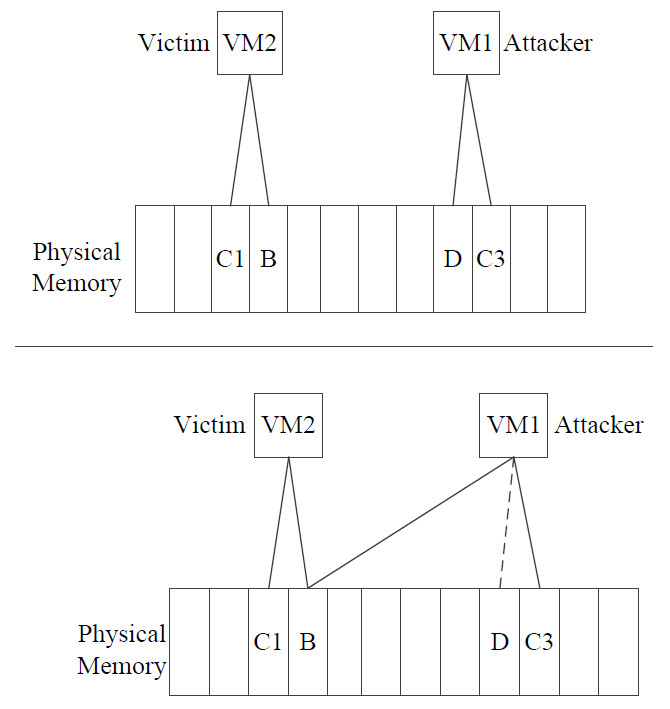
\includegraphics[width=8cm, height=7cm]{VMCS0.jpg}}%{pdfvmsm1.jpg}}
\caption{The execution process of double mapping. } \label{fig0}
\end{figure}

\textbf{Scene 2.}
    For the remapping attack, there are VM1 (attacker) and VM2 (victim). A physical page (A) used by VM2 is released after being used. After A is released, VM1 remaps to A. So that the guest virtual address of VM1 points to the physical page A. By this way, VM1 can access the information on A used by VM2, causing information leakage.

Through the analysis of these two kinds of attack models, it is necessary to achieve attack prevention through VM monitoring and VM isolation.
\subsection{Assumption}

We propose some assumptions.
%This paper focuses on the implementation of HyperMI. On the one hand, we assume that hardware is trusted. On the other hand, we do not take some attacks into account.
First, we assume hardware resources are trusted including processor, buses and so on, the trusted boot based on hardware can ensure the security and integrity of bootloaders. Obviously, the TCB contains created HyperMI and hardware resources. Second, this paper does not consider denial of service attack (DOS), side channel attack and hardware-based attack, such as cold-boot attacks and RowHammer.
% And we don't consider the attack incurred by interaction between VM and software with vulnerabilities.

%Our approach can avoid DMA (direct memory access) attack which can be used by attackers to break the isolation of HyperMI world. It can prevent attacker from implementing double mapping or remapping to memory page and cross-domain attack via VM monitoring. Besides, protection for critical interaction data between hypervisor and VM can prevent attacker from bypassing VM monitoring and implementing data leaking attack, even control flow hijack.

\iffalse
Our approach can resist these attacks including accessing any memory pages by page remapping or double mapping, malicious supervisor accessing to memory from hypervisor, malicious DMA (direct memory access) accessing and memory escalation attacks, etc. Besides, protection for critical interaction data between hypervisor and VM can prevent attacker from implementing data leakage attack, modifying special privilege register, even control flow hijack.
\fi

\section{Design}
In this section, we give the overview about the HyperMI architecture.% and describe the three important modules.


\subsection{Architecture} 
% To protect critical data in VM from being leaked, HyperMI is aimed to provide a secure isolated execution environment to protect running VM against compromised hypervisor without depending on the higher privilege level.

HyperMI is designed to provide a secure isolated execution environment to protect VM against compromised hypervisor without depending on a higher privilege level software than hypervisor or customized hardware.
\iffalse
The approach achieves three objectives: 1) A secure isolated environment at the same privilege level with hypervisor to host security tools with relatively trial performance overhead. 2) Completed secure memory isolation approach for VM to guarantee memory isolation against malicious memory access attack. 3) Non-bypassable secure runtime monitoring for interaction between hypervisor and VM when process exits from non-root mode to root mode. HyperMI also monitors access to VMCS data structure to finish context switching.
\fi


Figure \ref{fig1} shows the architecture, the overall system contains three parts: several isolated VMs, hypervisor either in normal world or in HyperMI word, memory hardware including HyperMI region for HyperMI world and normal region for normal world.

The origin hypervisor is divided into two parts: HyperMI world which security tools can run in and normal world which hypervisor runs in. Firstly, HyperMI world is used to run security tools when hypervisor is compromised, so that these tools running in secure HyperMI world can resist attacks from compromised hypervisor. Secondly, operations for EPT and context switching module are deprived from normal world for security, then are put into HyperMI world, but VM exit handler module is reserved to handle VM exit in normal world. Thirdly, these two worlds can communicate with each other through the only secure channel, named Switch Gate. 


\begin{figure}
\centerline{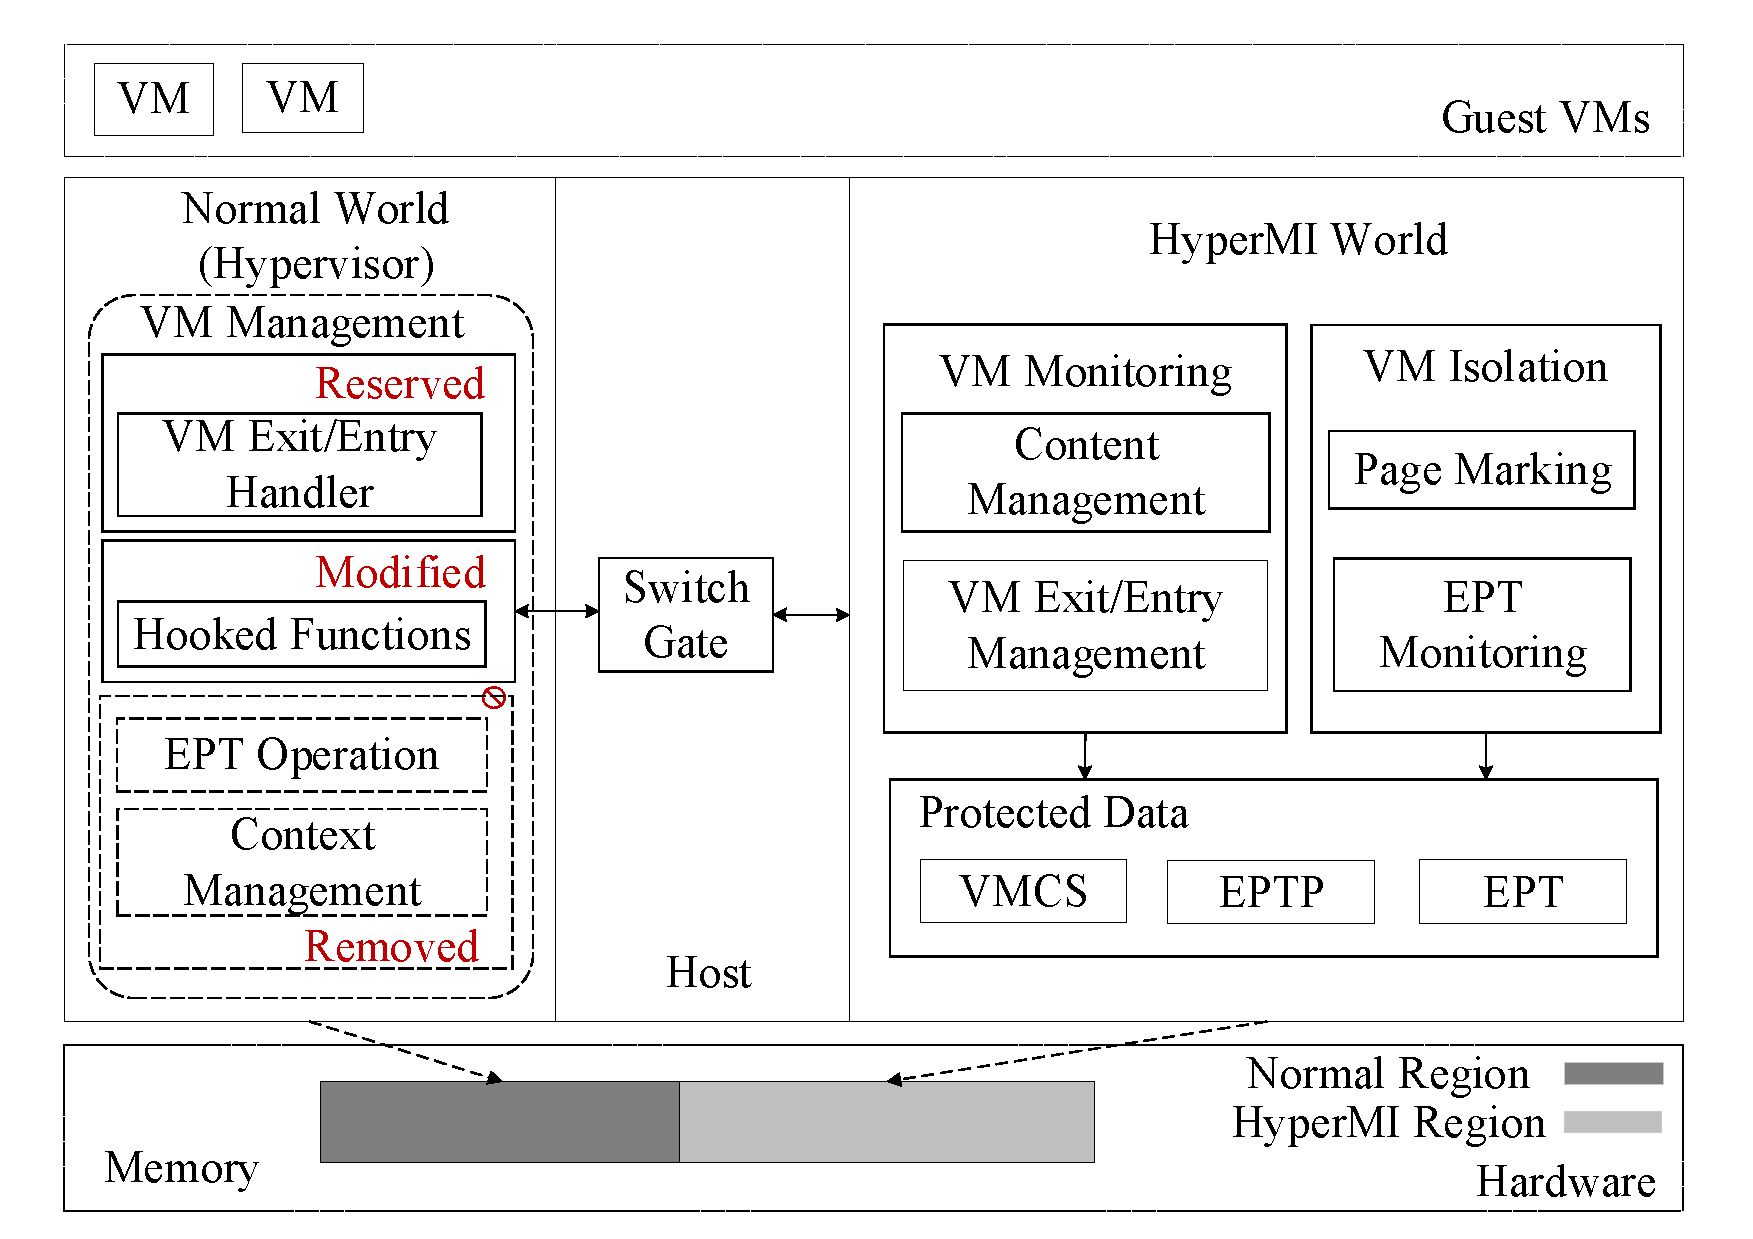
\includegraphics[width=9.5cm, height=7cm]{pdfvmcs1.pdf}}%{pdfvmsm1.jpg}}
\caption{The architecture of HyperMI. } \label{fig1}
\end{figure}

While the hypervisor together with guest VMs run in the normal world, the hypervisor is forced to request HyperMI to perform four operations on its behalf: 1) switching context between the hypervisor and VMs, 2) updating EPT of VMs, 3) verifying the pages when executing swapping operations to resist double mapping attack, 4) verifying the pages when executing releasing operations to resist remapping attack. After setting up the HyperMI, the whole system is ready to create isolated executing environment. With these designs, HyperMI enforces the isolation and protection of memory used by each VM. Furthermore, HyperMI guarantees security of interaction, memory isolation between the hypervisor and VMs.

\iffalse
In HW, operations for EPT and context switching module are deprived from normal world for security, then are put into HyperMI world, but VM exit handler module is reserved to handle VM exit in normal world. HyperMI world is created to place security tools including VM monitoring and VM isolation. For VM isolation, page marking module is used to mark physical memory pages when EPT updates and isolate memory among VMs. Also, protecting EPT and monitoring the related operations about EPT are provided by EPT monitoring module. For VM monitoring, we intercept the related functions about VMCS structure by setting hooks in normal world, then dispatch these functions to HyperMI world to handle, and monitor the interaction between hypervisor and every VM. Secondly, as long as the monitored event is triggered, these two worlds switch through the only secure channel, named Switch Gate. Thirdly, memory of the whole system is divided into two parts, memory of normal
region and HyperMI region. In the meantime, normal world can't access memory of HyperMI Region casually, which is isolated securely from normal region.
\fi

\subsection{Interaction}



Figure \ref{fig+1} shows the interaction process of HyperMI. 
\iffalse
We set the trigger by hooking the EPT operation and context switching function in Normal world. When these functions are called, HyperMI switch the control flow from Normal world to HyerMI world through the Switch Gate, then the security tools in HyperMI world performs the corresponding operations. VM Monitoring and VM Isolation finishes EPT operations and context switching. In addition, VM Isolation also divides memory into VM or hypervisor. When these operations are finished, the control execution flow returns to the normal world through the Switch Gate. 

\fi
In traditional system, VM interacts with hypervisor  by VM EXIT/VM ENTRY to request hypervisor to handle events. The execution process of the interaction is as follows. 1) VM switches context and exits to hypervisor. 2) Hypervisor handles the VM exit request events. 3)  Hypervisor executes VM resume instruction to entry VM.
In HyperMI system, HyperMI intercepts the VM exit request, executes context switch, to make sure interaction data not
be modified. The execution process of the interaction is as follows. 1) VM exits to HyperMI and switches context. 2) HyperMI exits to hypervisor. 3) Hypervisor handles the VM EXIT request events. 4) Hypervisor executes VM resume instruction to entry VM.

\fi
\iffalse
As described in the previous architecture, HyperMI is placed at the same privilege-level with hypervisor, but in different address space. The two worlds interact through the channel, switch gate.
In traditional system, VM interacts with hypervisor  by VM EXIT/ENTRY to request hypervisor to handle exit/entry events. The exit execution process is as follows. 1) VM requests to exit. 2) Switch context to store VM status. 3) Get VM exit reason information by accessing VMCS. 4) VM exits to hypervisor. 5) Hypervisor handles the VM exit request events. 
The entry exection proceess is in the reverse order. 1) VM requests to entry. 2) Switch context to store HOST status. 3) Hypervisor accesses VMCS. 4) Entry to VM.

%In HyperMI system, execution can be hijacked to HyperMI from hypervisor firstly, then return back to hypervisor.
In HyperMI system, HyperMI hooks interaction between VM and hypervisor funtcion, and address translation function (EPT updating) to deprive these two functions modules.
When these functions are called, the control flow is hooked to the HyperMI from hypervisor to HyperMI through the switch gate.
The exit execution process is as follows. 1) VM requests to exit. 2) Switch context to store VM status. 3) Get VM exit reason information by accessing VMCS in HyperMI world. 4) VM exits to hypervisor. 5) Hypervisor handles the VM exit request events. 
The entry exection proceess is in the reverse order. 1) VM requests to entry. 2) Switch context to store HOST status. 3) Hypervisor accesses VMCS in HyperMI. 4) Entry to VM.


% 3) Hypervisor executes VM resume instruction to entry VM.

\begin{figure}
\centerline{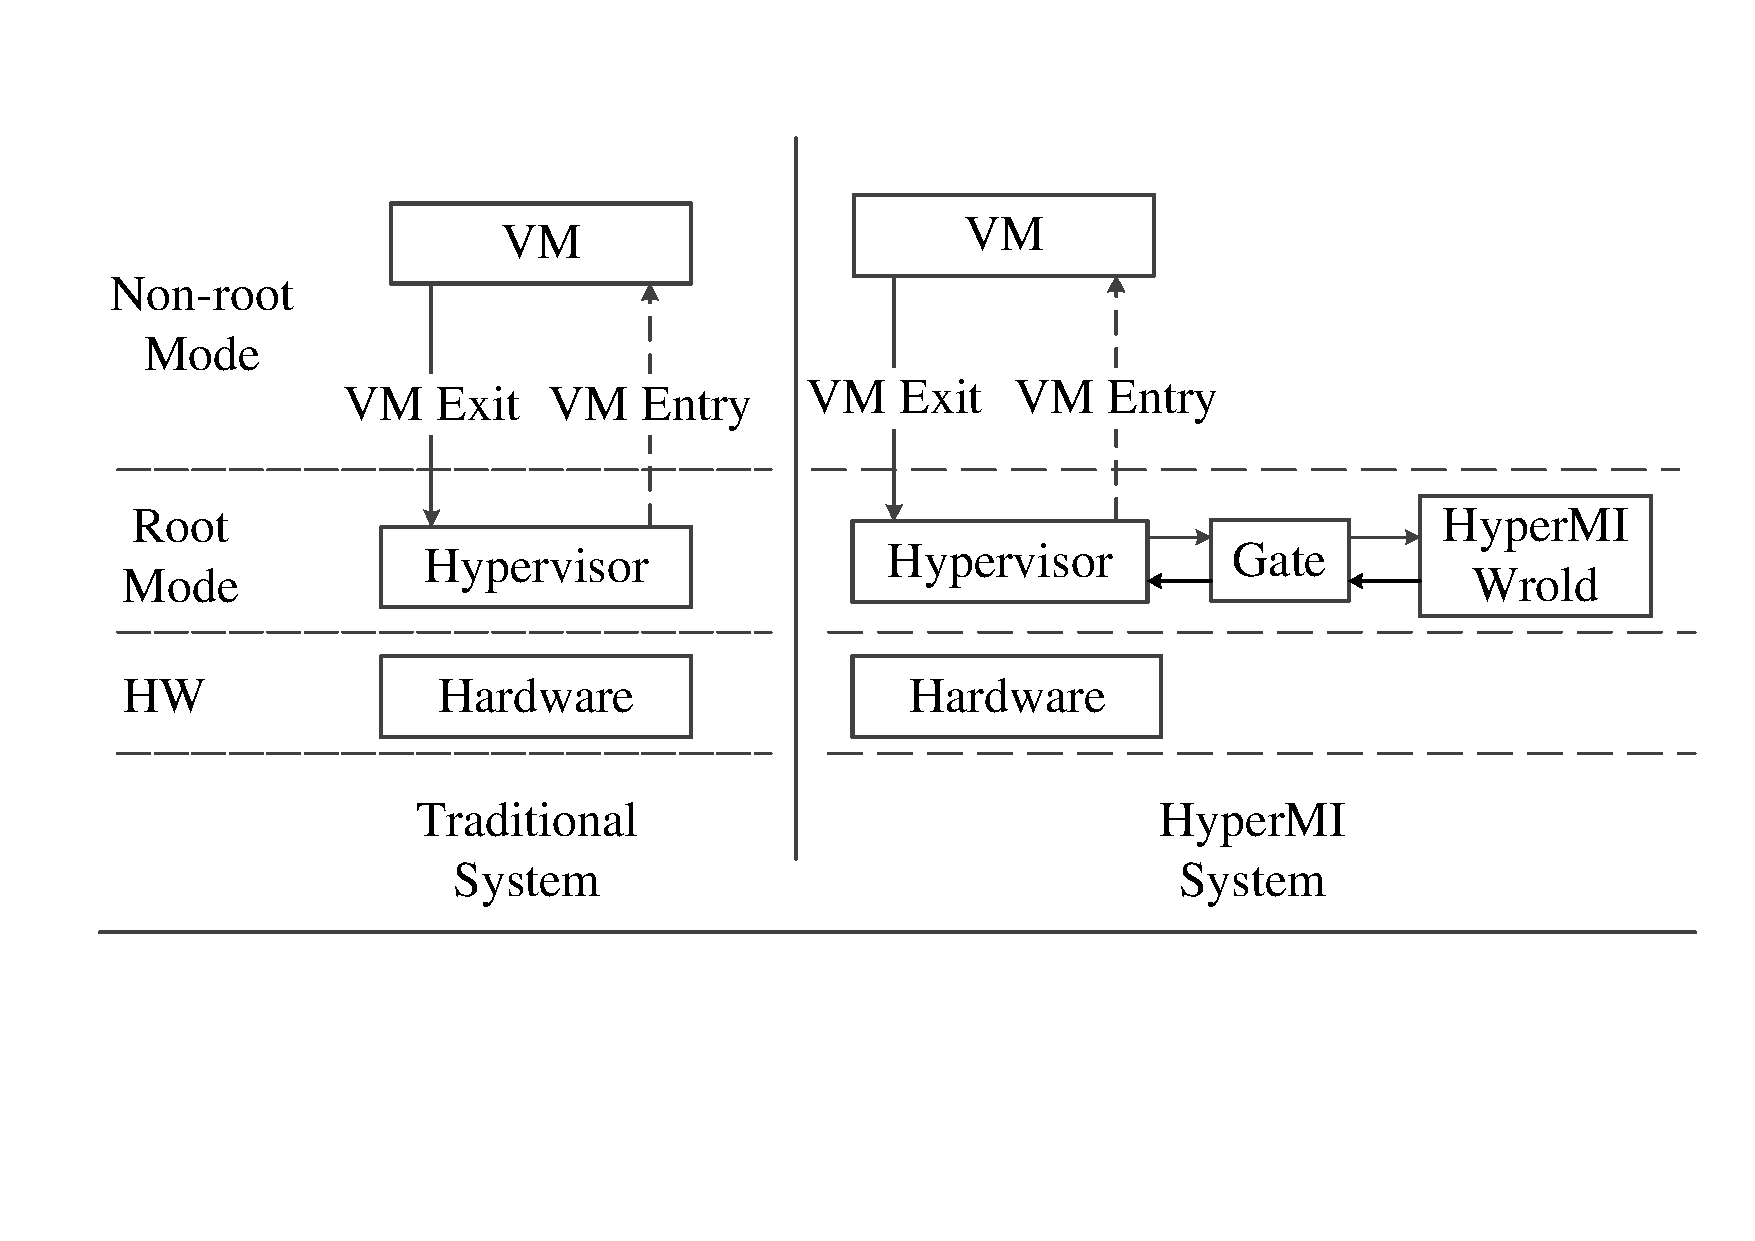
\includegraphics[width=9cm, height=5.5cm]{pdfvmcsProcess.pdf}}
\caption{Interaction of HyperMI. } \label{fig+1}
\end{figure}


\section{Implementation}

HyperMI is implemented on x86 platform base on KVM.
We describe the implementation of key components in the HyperMI architecture below including HyperMI world, VM monitoring and VM isolation.

%\subsection{Secure Isolated execution Environment}
\subsection{HyperMI World} \label {HWorld}
HyperMI world, as a secure isolated execution environment, is created to place security tools to resist compromised hypervisor against leaking information, accessing data illegally and falsifying data. 
%In the meantime, efforts must be adopted for the security of this environment. 
In order to make sure the isolation and security of HyperMI world, we implemented the following three strategies.
Firstly, to achieve isolation, HyperMI world is created on another kernel page table, so that normal world can't access HyperMI world. Secondly, the only and secure switch gate is required to provide switch channel for two different worlds. The switch gate is the only channel to avoid bypassing HyperMI world attack. The gate is secure by using atomic operation to avoid the address of HyperMI world leakage attack. Thirdly, some secure approaches must be adopted to protect HyperMI world against bypassing HyperMI world and breaking HyperMI world. Because attackers can load new page table and bypass HyperMI world by modifying the value of register CR3, attack running HyperMI world while the code in normal world has executive privilege.

\begin{figure}
\centerline{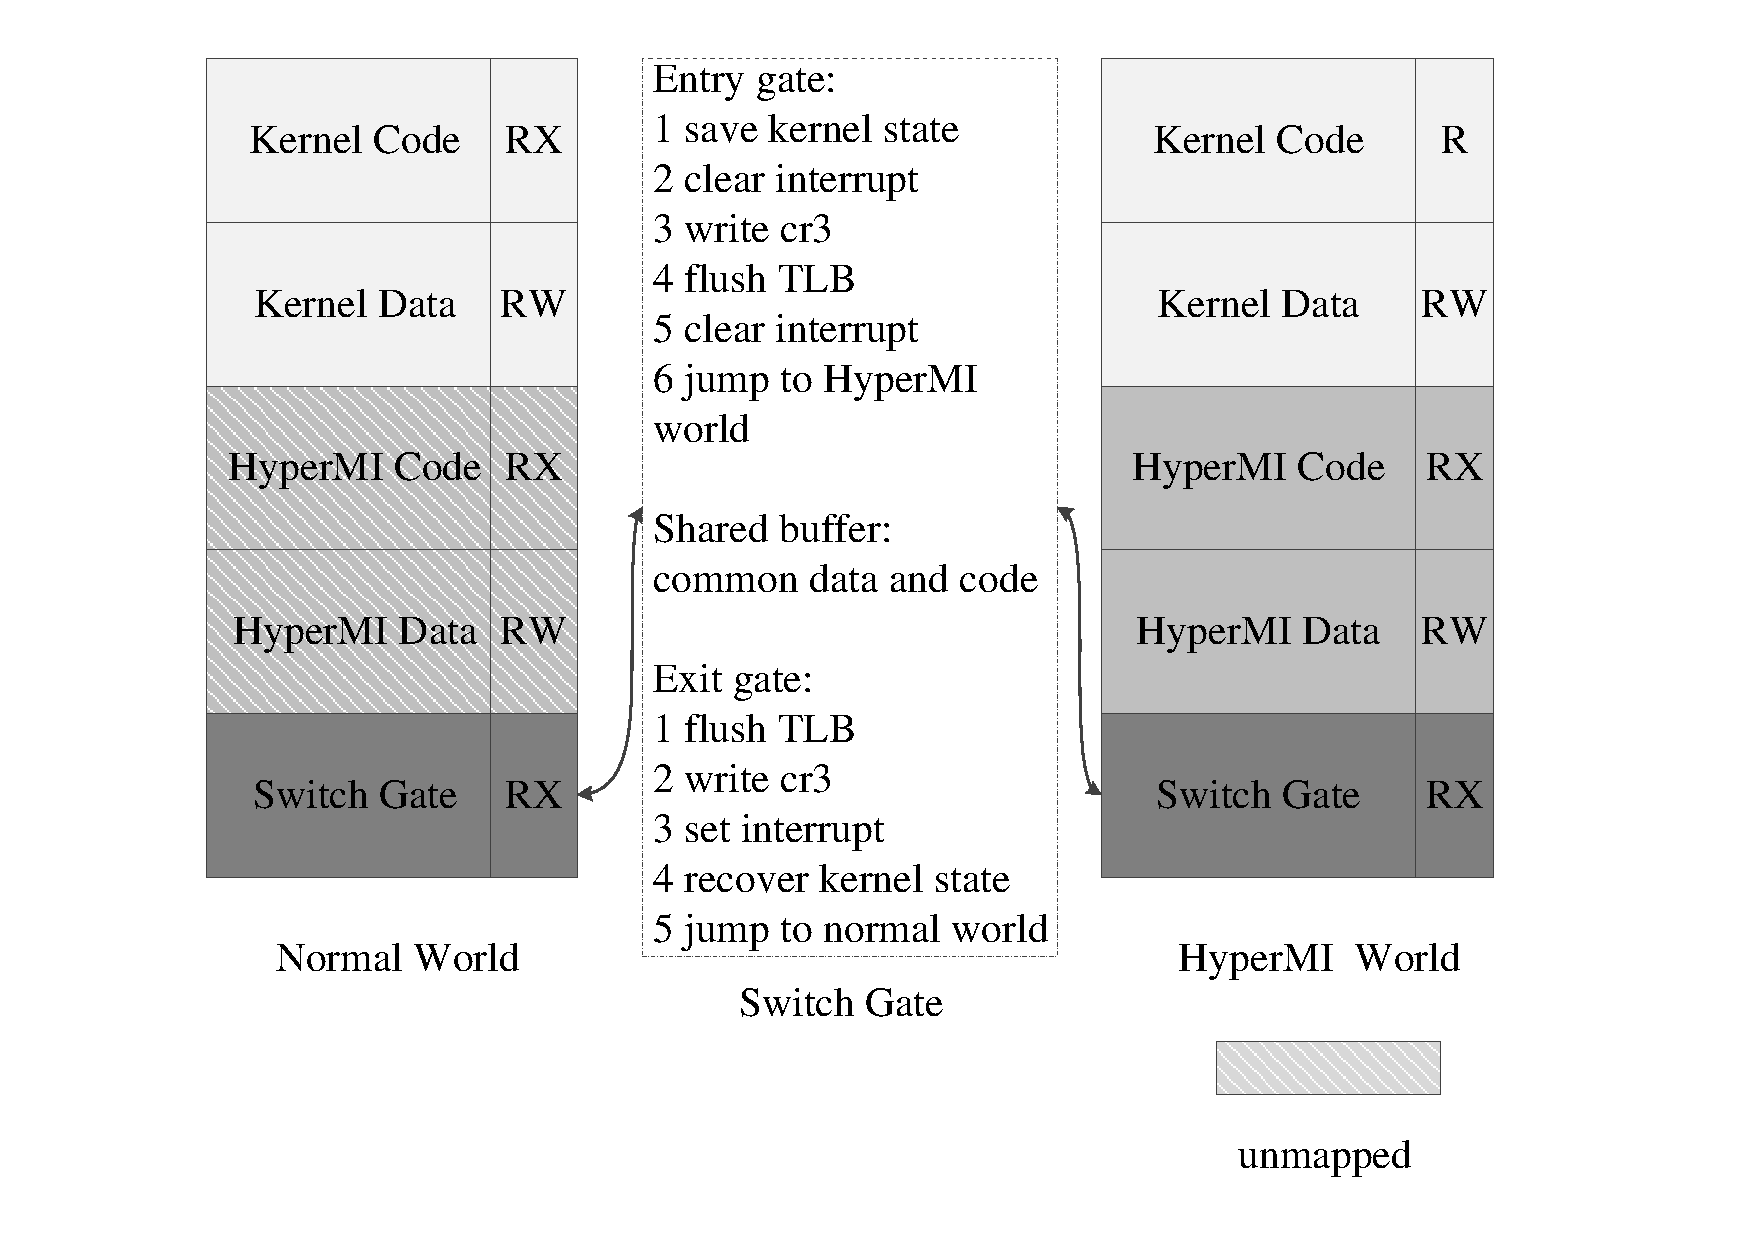
\includegraphics[width=11cm, height=8cm]{pdfvmcs2.pdf}}%{vmsm23.jpg}}
\caption{An overview of address space layout.} \label{fig2}
\end{figure}


\textbf{Creation of HyperMI World}
HyperMI world is created to provide a secure execution environment for security tools against compromised hypervisor. To satisfy isolation, the code and data segment of HyperMI world must not be accessed by compromised hypervisor. We use two isolated address space based on two sets of page table to achieve isolation.
Figure \ref{fig2} describes the address space layout of two worlds through two sets of page table, the normal page table and the secure page table. On the left of Figure \ref{fig2}, the normal page table contains address of the normal world except for address of HyperMI world in case of compromised hypervisor breaking the integrity of code and data in HyperMI world. Program running in normal world cannot access data in HyperMI world. On the right of Figure \ref{fig2}, all address are mapped in this secure page table.
HyperMI code remains executable and HyperMI data remains writable. Kernel code is forbid to execute with reference to protection for running HyperMI world. 
In the middle of Figure \ref{fig2}, the switch gate includes entry/exit gate and shared buffer. Entry gate provides the only entrance to HyperMI world while the exit gate provides the address to return to the normal space. Shared buffer contains common data and code which the system needs to run the switch process. Common code is switch code, common data is entrance address to HyperMI world and return address to normal world. The switch gate is mapped at the same place in the normal world and HyperMI world because the page table loading code must be called by the two worlds before and after switching. Of course, the entrance address must be protected after switching to HyperMI world in case of malicious attacker accessing HyperMI world causally after trusted boot. 



Obviously, HyperMI world is based on page table. There are three reasons for controlling the two set of kernel page tables: 1) To access casually or bypass HyperMI world, attacker can tamper the content of page table to map to the physical page belonging to HyperMI world or load malicious page table to CR3. 2) To execute code injection attack, attacker can close the write protection mechanism by modifying the value of CR0 register, changing the access permission bits of the memory page. Then cover the hooked functions we use, redirect the functions to their own malicious code and bypass secure monitoring of HyperMI. 3) To break HyperMI world, attacker can access HyperMI world causally when HyperMI world is running if kernel code has the execution permission. Therefore, three secure approaches against these attacks are as follow.

For the first attack, we make some segment unmapped by creating another page table, named secure page table, which contains HyperMI code and data. And to protect the entrance address to HyperMI world from being leaked,
%pre-allocate some space during trusted boot which kernel can't access directly through MMU, critical data in
remove all entries that map to HyperMI world from the page table in normal world. Deprive the ability of accessing CR3 of kernel in order to avoid to load illegal page table, and resist bypassing HyperMI world.
For the second attack, intercept the accessing operation to CR0 and maintain the WP bit as 1. Stick to W$\oplus${X} mapping and code segment belonging to hooked functions still maintains unwritable.
To go against the third attack, we set the kernel code segment as NX (non-executable) when HyperMI world is running. For more security, modify the kernel to configure all page tables as read-only by setting access permission bits of specific page table entries mapping to the memory regions of the page tables. This is necessary to prevent the page tables from being compromised by attackers. Any access permission modification to kernel page tables must cause the kernel to page fault, then we dispatch page fault to HyperMI world to handle.

\textbf{Worlds Switch}
HyperMI creates a switch gate for switch between normal world and HyperMI world by loading a page table of the next space into CR3. And we must ensure atomicity and security during the switching process.

The switching process described in Figure \ref{fig2} is as follow: 1) Save the kernel state to the stack including generic registers and interrupt enable / disable status. 2) Clear the interrupt with the CLI instruction. 3) Load the page table to the register CR3 and flush the TLB. 4) Interrupt again. 5) Jump to the HyperMI region. For the exit process, return to the normal world by performing the operations in the reverse order.

During this switching process, attackers can attack the system by violating atomicity and security. 1) Interrupt the gate's execution sequence and violate the atomicity. 2) Jump the first interrupt and get the base address of page table of HyperMI world after writing to CR3 can go against security. Therefore, interrupt policy is used to guarantee atomicity and twice interrupt is required to ensure security in case of attacker carrying out attack after getting the address of HyperMI world. Saving the kernel state can make running program return to normal world normally. 

\subsection{Security Guarantee for HyperMI World}\label {SG}
Nevertheless, without any protection measures, the page table to load to switch to HyperMI world is not secure for three reasons: 1) Hypervisor with the highest privilege can control page table. 2) Free to execute privileged instructions. 3) Carry out DMA attack to access HyperMI world casually.

Firstly, hypervisor has full control of page tables, so it can attack the HyperMI world. Actually, protection for page tables is detailed in section \ref{HWorld}. 

Secondly, hypervisor is still privileged and it can free to execute privilege instructions, so it can write any value to the related privileged registers. 1) Malicious attackers can close DEP mechanism by writing to CR0, close SMEP mechanism by writing to CR4. 2) Kernel code can load a crafted page table to bypass the HyperMI world by converting a meticulously constructed address of one page table to CR3.
Actually, to protect the system, HyperMI deprives sensitive privileges instructions executed by hypervisor, and dispatches the captured events to the HyperMI world. The HyperMI world can choose how to handle this event, such as issuing alerts, terminating the process, or doing nothing. The whole process is similar to the signal handling in traditional OSes.

Thirdly, it is important to focus on DMA attack. DMA operation is used by hardware devices to access physical address directly. Malicious attackers can read or write arbitrary memory regions including HyperMI world by DMA. Therefore, it is a key focus of intercepting access to physical pages belonging to HyperMI world directly by DMA operation. 
Fortunately, HyperMI employs IOMMU mechanism to avoid DMA attack, which can carry out access control for DMA access. Our approach adopts two policies: 1) Remove the corresponding mapping of the critical data from the page table which IOMMU uses. These critical unmapped data includes the entrance address of HyperMI, data recording Page-Mark structure used in VM isolation, VM-Mark structure used in VM monitoring and so on. 2) Intercept the address mapping functions about I/O, verify whether the address is in address space of HyperMI world, then choose to map or unmap.


%\subsection{VM Isolation and Monitoring }



\subsection{VM Monitoring}

During the VM entry/exit process, the related state information of every virtual CPU and host OS are stored in VMCS structure. 
And only the VMX root privilege instructions, such as VMPTRLD, VMPTRS, VMCLEAR, VMWRITE and VMREAD, can operate the VMCS.
% And the related operations about VMCS are VMPTRLD, VMPTRS, VMCLEAR, VMWRITE and VMREAD.
VM exit is a point to intercept accessing operation of VMCS. HyperMI intercepts and validates interaction between hypervisor and VM: 1) Interception of context switching. 2) VM exit redirection.

\textbf{Interception of Context Switching}
Obviously, the protection to VMCS structure can't be ignored based on the fact that VMCS is structure recording all context informations of the VM and it is managed by the compromised hypervisor. 
% Obviously, when hypervisor interacts with VM, the protection for VMCS structure can't be ignored.
The VMCS structure always records the information of privileged registers, such as HOST\_CR3, EPT\_POINTER, HOST\_CR0, HOST\_CR4, VM\_EXIT\_MSR\_STORE\_ADDR, HOST\_RIP and so on. During the VM entry or VM exit, the compromised hypervisor can tamper VMCS structure, so the system can suffer these attacks: 1) Access memory region of VMCS directly. 2) Falsify the value of HOST\_RIP, and the system will suffer control flow hijack. 3) Tamper the value of EPT\_POINTER(EPTP), and other malicious EPT is loaded. 4) Fake the value of HOST\_CR3, so the page table of host OS can be replaced.

For the first kind of attack, to prevent compromised hypervisor accessing memory region of VMCS structure, HyperMI hides the base address of VMCS structure in HyperMI world. So, hypervisor loses the ability of accessing VMCS structure. To ensure the system run normally, hypervisor must require HyperMI to return the signal information rather than real address on demand or trap the functions to the HyperMI world, and avoid many functions about VMCS operations to access the address of VMCS structure directly. To avoid the last kind of attack, in addition to hiding the address, HyperMI also intercepts and validates the execution of these instructions by placing hooks at these functions (vmcs\_writel, vmcs\_readl et al.). So hypervisor requests HyperMI world to handle operations about VMCS and return corresponding result for legal request, as Figure \ref{fig4} shows.

\textbf{VM Exit Redirection}
% VMCS structure can only be accessed in two time quantum, VM exit and VM entry.
% VMCS structure is accessed during only two time quantum, VM exit and VM entry.
VMCS structure can only be accessed during VMX root operation, therefore, the switching point between VMX Non-Root operation and VMX Root operation provide HyperMI a perfect point to perform security check. In details, HyperMI would intercept the process of VM Exit and redirect to HyperMI world to perform security check. 
% And the data of VMCS structure is the same during VM exit and VM entry. So we choose VM exit as a time point to intercept VMCS structure. Only when VM exit, can hardware data structure have great significance.
% During the VM entry/exit process, the related state information of every virtual CPU and host OS are stored in VMCS structure. And the related operations about VMCS are VMPTRLD, VMPTRS, VMCLEAR, VMWRITE and VMREAD. VM exit is a point to intercept accessing operation of VMCS. HyperMI intercepts and validates interaction between hypervisor and VM: 1) Interception of context switching. 2) VM exit redirection.
%
% \textbf{Interception of Context Switching}
% Obviously, when hypervisor interacts with VM, the protection for VMCS structure can't be ignored. It always records the information of privileged registers, such as HOST\_CR3, EPT\_POINTER, HOST\_CR0, HOST\_CR4, VM\_EXIT\_MSR\_STORE\_ADDR, HOST\_RIP and so on. During the VM entry or VM exit, the compromised hypervisor can tamper VMCS structure, so the system can suffer these attacks: 1) Access memory region of VMCS directly. 2) Falsify the value of HOST\_RIP, and the system will suffer control flow hijack. 3) Tamper the value of EPT\_POINTER(EPTP), and other malicious EPT is loaded. 4) Fake the value of HOST\_CR3, so the page table of host OS can be replaced.
%
% For the first attack, to prevent compromised hypervisor accessing memory region of VMCS structure, HyperMI hides the base address of VMCS structure in HyperMI world. So, hypervisor loses the ability of accessing VMCS structure. To ensure the system run normally, hypervisor must require HyperMI to return the signal information rather than real address on demand or trap the functions to the HyperMI world, and avoid many related functions to access the address of VMCS structure directly. To avoid the last three attacks, besides hiding the address, HyperMI also intercepts and validates the execution of these instructions by placing hooks at these functions (vmcs\_writel, vmcs\_readl et al.). So hypervisor requests HyperMI world to handle operations about VMCS and return corresponding result for legal request, as Figure \ref{fig4} shows.
%
% \textbf{VM Exit Redirection}
% VMCS structure is accessed during only two time quantum, VM exit and VM entry. And the data of VMCS structure is the same during VM exit and VM entry. So we choose VM exit as a time point to intercept VMCS structure. Only when VM exit, can hardware data structure have great significance.
%
To intercept the context switching efficiently, HyperMI chooses a novel way showed in Figure \ref{fig4}. Firstly, trap events of VM exit, when VM exit events happen, HyperMI saves the hypervisor states firstly for security and then dispatches exit events to hypervisor to handle. To cut down the performance overload, HyperMI set VM exit configure of conditional exit events as non-running and reduce the occurrence number of exit events.

\begin{figure}
\centerline{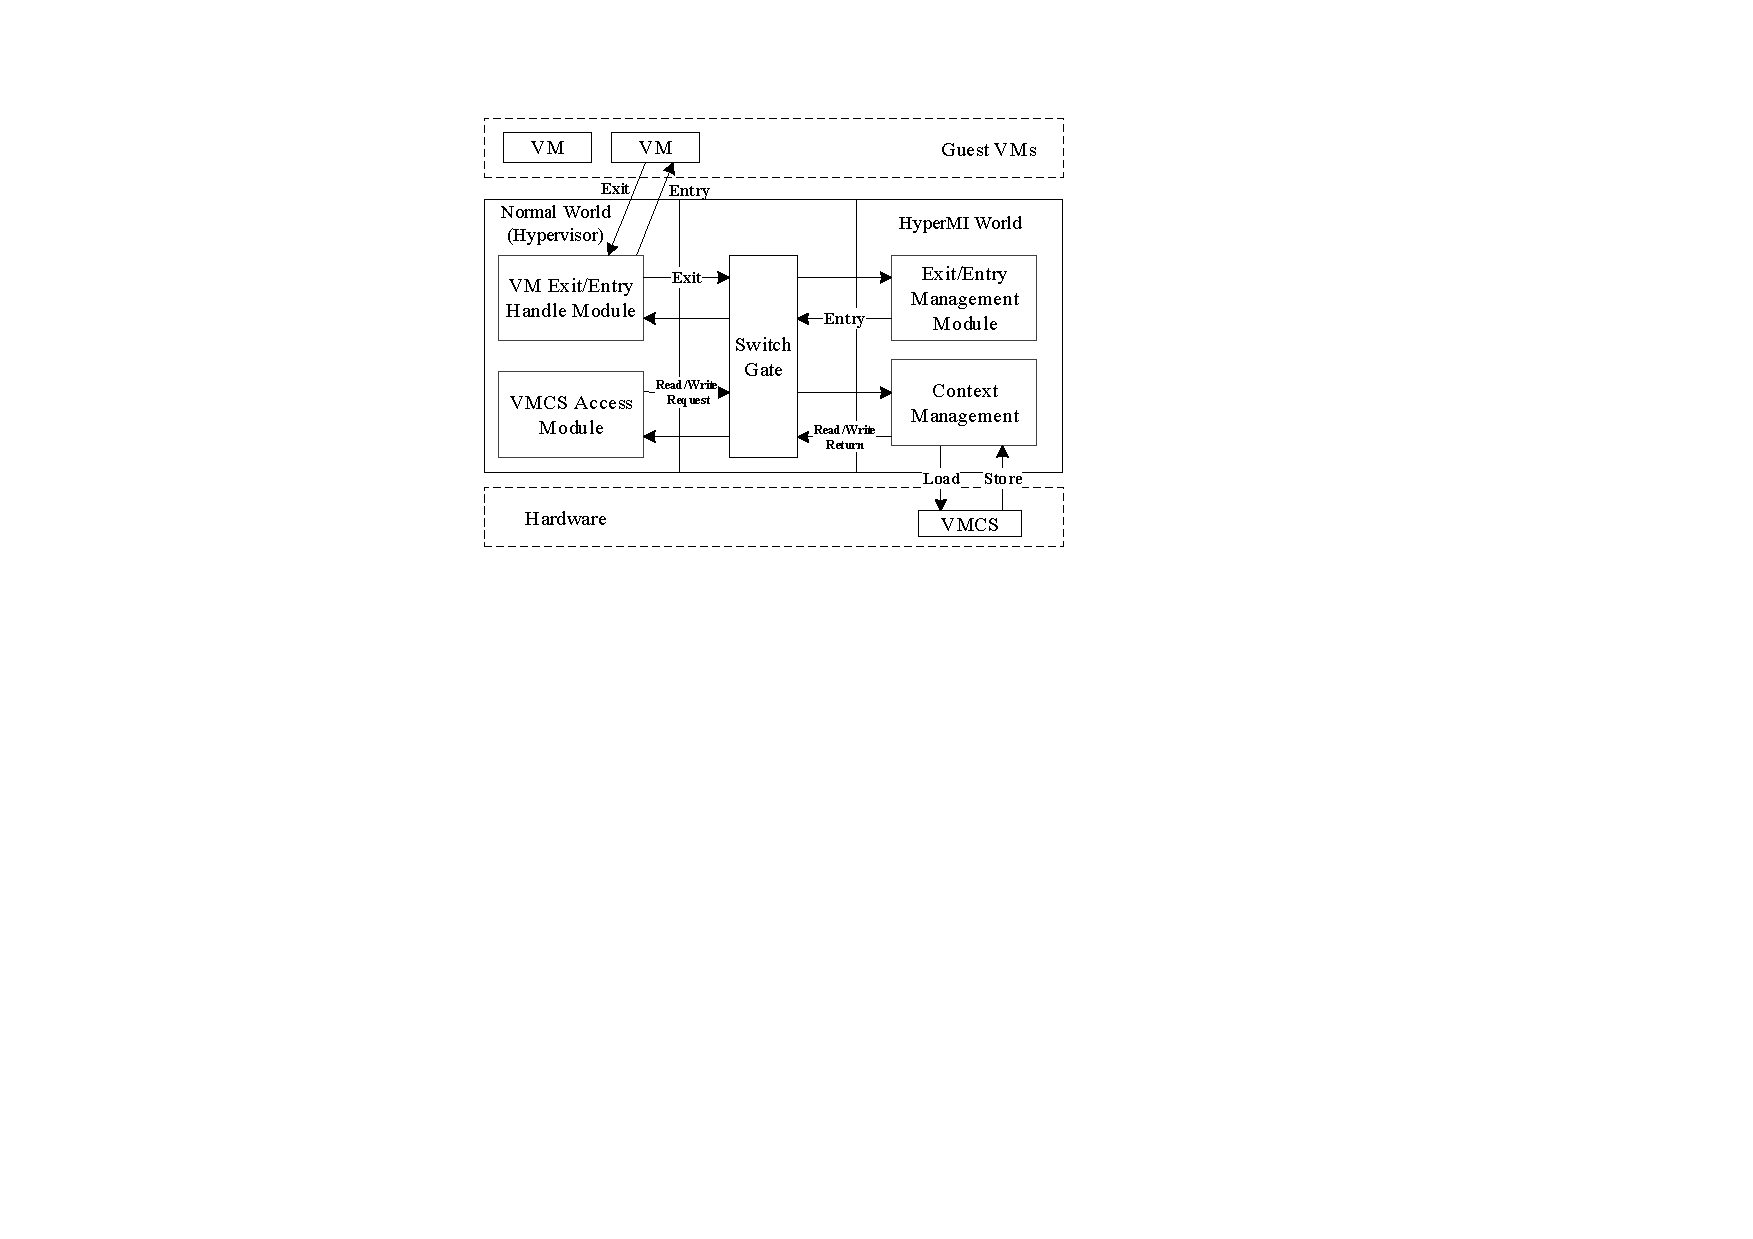
\includegraphics[width=9cm,height=6.5cm]{pdfvmcs4.pdf}}%{vmsm43.jpg}}
\caption{An overview of VM monitoring.} \label{fig4}
\end{figure}







\subsection{VM Isolation}\label{VMISolation}
% Hypervisor takes over all the memory pages with highest privilege level. When a VM accesses a page firstly, page fault is triggered and hypervisor finishes address translation from GPA to HPA through EPT. So all page access operations must need the help of EPT to finish page mapping. It is important to control page mapping when EPT updates. To achieve the goal of VM isolation completely, we adopt the approach that mark memory page with flag and track the page. However, a time point is needed for marking all page. And it is no doubt that EPT updating is a great point because hypervisor can manage all page mapping efficiently when EPT updates. Besides, EPT must be protected in case of data being leaked because EPT plays an important role in address translation of VM. So we describe VM isolation in these two aspects, EPT interception and memory isolation for VM.

As known to all, when Intel VT-d is enabled, all the physical memory is managed by the hypervisor using Extended Page Tables (EPTs), EPTs must be involved in each memory access and determine the permissions of the accessed memory page frame. Besides, the hypervisor employs different EPTs to manage the corresponding physical memory area for different VMs. If the page is remapped or double mapped, the system causes page fault. Page is accessed by VM through EPT updating.
% becuase different VMs share the same physical memory
%Especially during the initialization, the hypervisor takes charge of establishing all memory mapping and filling all EPT Entries for all available memory page frame. Thus, 
% Hypervisor takes over all the memory pages with highest privilege level. When a VM accesses a page firstly, page fault is triggered and hypervisor finishes address translation from GPA to HPA through EPT. So all page access operations must need the help of EPT to finish page mapping.
it is important to control page mapping when EPT updates. To achieve the goal of VM isolation completely, we adopt page marking technique, that marks memory page with flag and track the page. However, a time point is needed for marking all page. And it is no doubt that EPT updating is a great point because hypervisor can manage all page mapping efficiently when EPT updates. Besides, EPT must be protected in case of data being leaked because EPT plays an important role in address translation of VM. So we describe VM isolation in these two aspects, EPT interception and memory isolation for VM.


\textbf{Interception of EPT Operation }
During the translation process of mapping GPA to HPA through EPT, a VM can suffer these attacks: 1) Compromised hypervisor can access EPT of every VM, then does whatever it wants by modifying the address mapping causing remapping and double mapping attack. 2) Load the malicious EPT and execute illegally.

Confronting with these attacks, we can see that the ultimate purpose of attackers is to access the physical memory page frames of other VM. HyperMI solves the issue using the following policies: 1) Hide the address of EPT and make it unmapped for kernel in normal world. 2) Intercept the related operations including EPT creating, loading, updating, walking and destroying to avoid leaking the address of EPT. 3) Mark respective EPT for every VM, isolate EPT among VMs, and ensure that the right and corresponding EPT is loaded for every VM.




\begin{table}[htbp]
\centering
\caption{VM-Mark Table.}\label{tab1}
%\begin{tabular}{c|c|c|c}
\begin{tabular}{p{1.4cm}|p{1.2cm}|p{1.1cm}|p{1.7cm}}
\hline
\multicolumn{4}{c}{\bfseries\textbf\centering{VM-Mark Table}}\\
\hline
{\itshape\bfseries Label} & VMID & EPTID & EPT\_Address\\
\hline
{\itshape\bfseries Description} & { The VM Identifier} & The EPT Identifier & The Entry Address of EPT\\
\hline
\end{tabular}
\end{table}

% For the first policy, the address of EPT can be stored in two places, one is created in creating EPT function, a software operation, the other is recorded in EPTP, a hardware data unit in VMCS structure. Therefore, it is critical to intercept the EPT creating operation and store the address of EPT in HyperMI world. Specially, store VMCS structure including EPTP in HyperMI world. However, some functions need the address of EPT to perform. There is a novel idea that HyperMI returns signal information necessarily to these functions rather than true address to make the system run normally.
% For the first policy, the address of EPT can be stored in two places, one is created in creating EPT function, a software operation, the other is recorded in EPTP, a hardware data unit in VMCS structure.
For the first policy, three places should be particularly protected. The first place is the EPT creation function where the function would return a CR3-like address: EPTP value. The second place is VMCS where would record the value of corresponding EPTP. The last place is the hardware register EPTP, the work of this register is similar to that of the CR3 register, which is used to provide MMU with the location of EPT. 
Therefore, it is critical to intercept the EPT creating operation and protect the stored address of EPT in HyperMI world. Especially, it is important to store VMCS structure who contains the value of EPTP in HyperMI world. 
%Specially, store VMCS structure including EPTP in HyperMI world. 
% However, some functions need the address of EPT to perform.
However, some functions, in addition to the EPT creation function, still rely on the value of EPTP. In this paper, HyperMI provides a novel approach that HyperMI returns signal information necessarily to these functions rather than true address to make the system run normally. 
% There is a novel idea that HyperMI returns signal information necessarily to these functions rather than true address to make the system run normally.
For the second policy, some functions, EPT creating, loading, walking and destroying, need access address of EPT. HyperMI places hooks on these functions, then dispatches them to HyperMI world and handle appropriately. In the meantime, HyperMI handles double mapping to ensure that there is only one virtual address mapping to one physical memory page during the EPT updating, and handles remapping problems to ensure the content of page cleaned after page being swapped out. This will be described in detail later.
\begin{figure}
\centerline{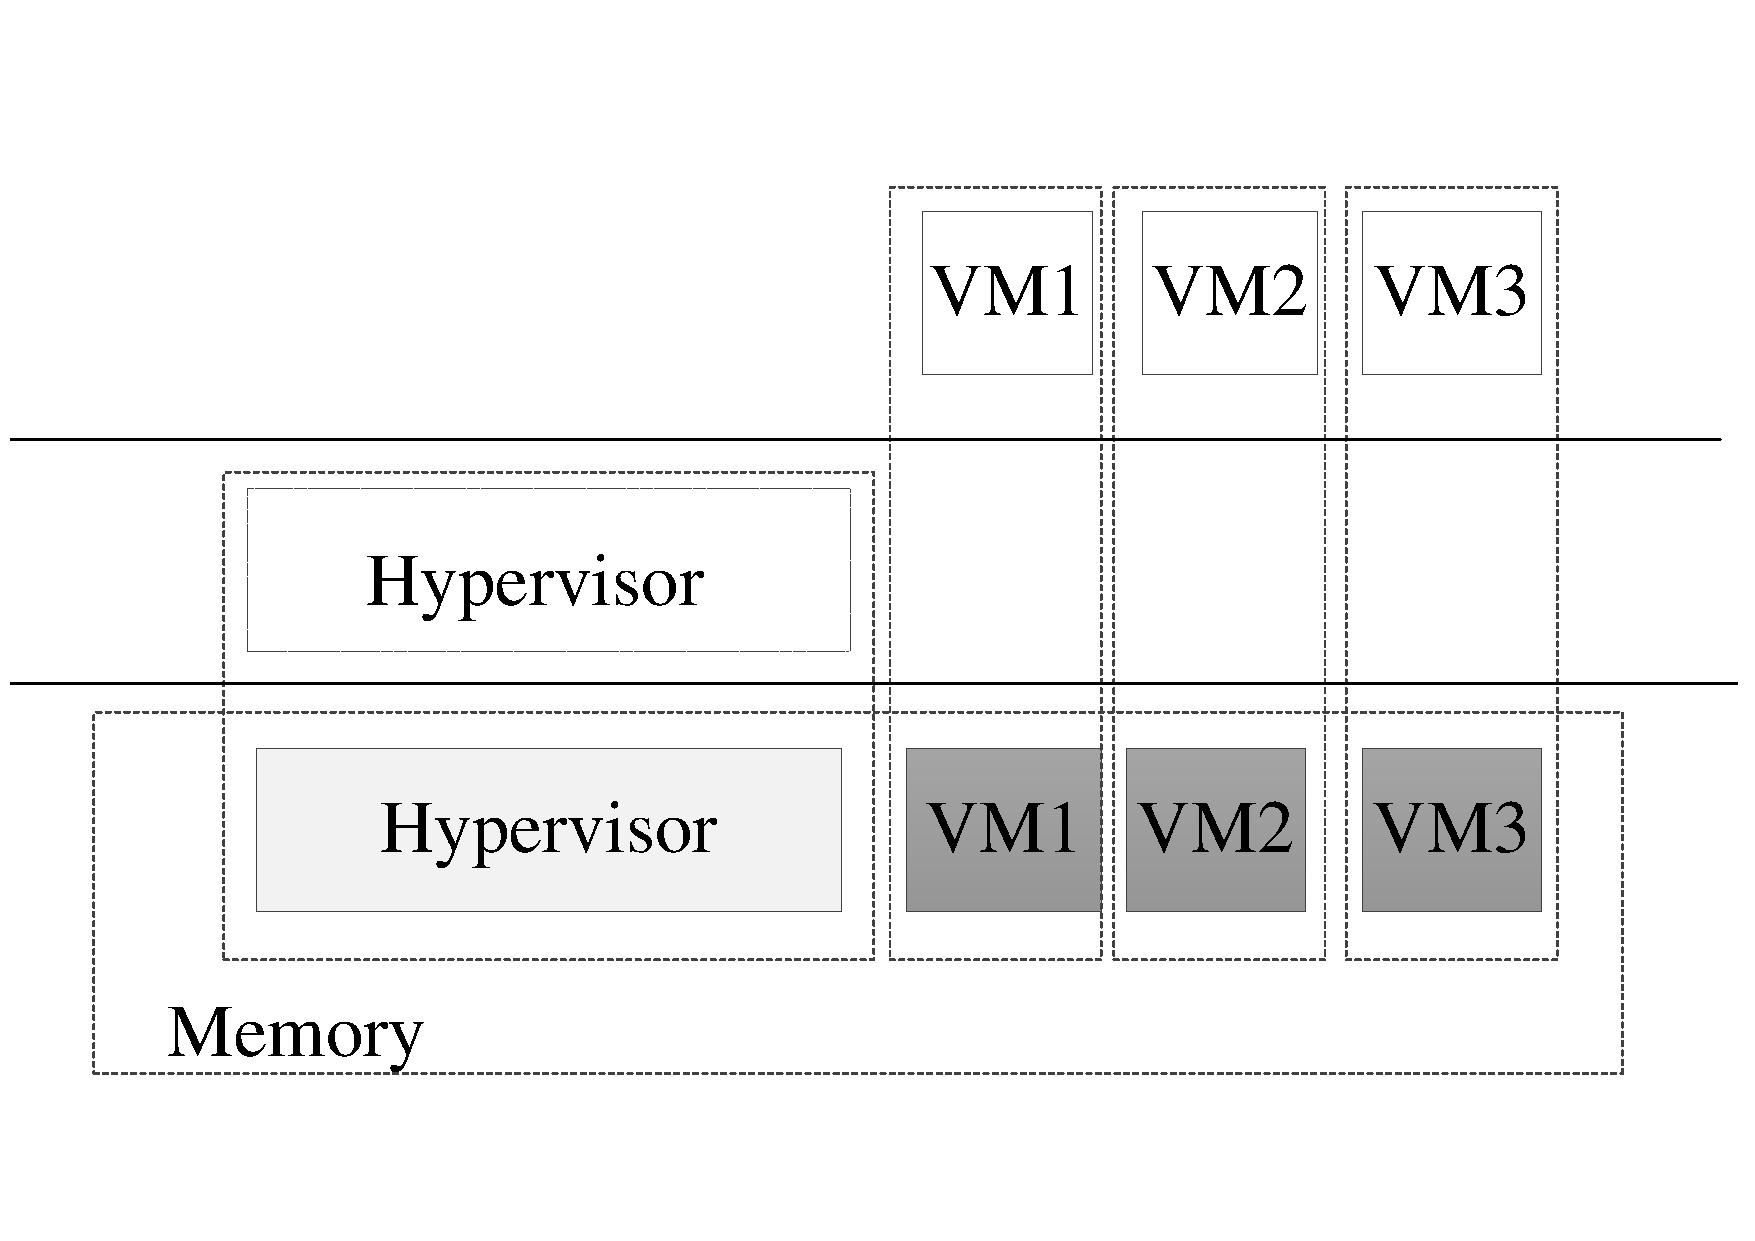
\includegraphics[width=9cm, height=6cm]{pdfvmcs3.pdf}}%{vmsm32.jpg}}
\caption{Memory isolation for VM.} \label{fig3}
\end{figure}
For the last one, intercepting the loading EPT operation and verifying the correctness of EPT can avoid loading a wrong EPT and leaking the content of physical memory page. To ensure one EPT for one VM, HyperMI creates the VM-Mark structure stored in HyperMI world as Table 1 described, and record VMID, EPTID, EPT\_Address and binds them together. VMID is created and destroyed based on hash value of image of VM. EPTID and EPT\_Address is recorded as long as the EPT of current VM is created.

\textbf{Memory Isolation for VM }
% Besides isolated EPT above, it should be considered that isolate memory to achieve the goal of VM isolation completely, as Figure \ref{fig3} describes. Hypervisor and every VM just can access own physical memory. Without memory isolation mechanism, compromised hypervisor and compromised VM can access memory pages of victimized VM by two ways when EPT updates: 1) Double mapping. 2) Remapping to pages with content. So some efforts are done. Monitor EPT updating and create Page-Mark structure described in Table 2 to record the owner of every physical memory page.
In addition the isolation EPTs mentioned above, isolating memory is another aspect that should be considered to achieve the goal of VM isolation completely, which is depicted in Figure \ref{fig3}. 
% Besides isolated EPT above, it should be considered that isolate memory to achieve the goal of VM isolation completely, as Figure \ref{fig3} describes.
Hypervisor and every VM just can access own physical memory. Without memory isolation mechanism, compromised hypervisor and compromised VM can access memory pages of victimized VM by two ways when EPT updates: 1) Double mapping. 2) Remapping to pages with content. So some efforts are done. Monitoring EPT updating and creating Page-Mark structure described in Table 2 to record the owner of every physical memory page. 

\begin{table}
\centering
\caption{Page-Mark Table.}\label{tab2}
%\begin{tabular}{|c{1cm}|c|c|c|}
\begin{tabular}{p{1.2cm}|p{1.4cm}|p{1.2cm}|p{1.5cm}}
\hline
\multicolumn{4}{c}{\bfseries\textbf\centering{Page-Mark Table}}\\
\hline
{\itshape\bfseries Label} & OwnerID & SharedBit & Used \\
\hline
{\itshape\bfseries Description} & The Owner Identifier & Shared or Unshared & Free or Used \\
\hline
\end{tabular}
\end{table}



% To go against double mapping during the process of EPT updating, HyperMI should finish these two tasks: verify the owner of pages firstly, and then mark OwnerID of Page-Mark structure for unused pages or thwart the mapping operation for used pages in case of malicious double mapping behavior. So the technique of pages allocation can divide all the pages into the pages of hypervisor or the pages of every VM.
%
% To go against remapping, HyperMI cleans the context of the page when the page is swapped out, so attackers can't get the context of the page by the way of remapping. And HyperMI marks the Page-Mark structure of corresponding page unused. This solution is the same as the treatment method of pointer for the purpose of security protection.
%
% Besides, for the page sharing feature of the system, it may hinder the implementation of the above measures. Confronting with this trouble, HyperMI deprives the shared page setting function and sets the corresponding bit in Page-Mark structure. The approach is detailed as follow: 1) Hypervisor requests HyperMI to return the hash map array (page frame number and hash value based on content). 2) HyperMI collects the hash array with considering that the same content results in the same hash value. 3) Hypervisor gets the hash array, finds the pages, then updates stable tree and unstable tree. 4) Hypervisor requests HyperMI to merge the page and set the SharedBit flag of the corresponding physical memory page. HA-VMSI \cite{Zhu2017HA} has a similar way with this idea.
%

In order to against the double mapping attack in the process of EPT updating, HyperMI should finish these two tasks: verifying the owner of pages firstly, and then marking the OwnerID of Page-Mark structure for unused pages or thwart the mapping operation for used pages in case of malicious double mapping behavior. So the technique of pages allocation can divide all the pages into different catalogues: the pages of hypervisor or the pages of every VM.

To go against the remapping attack, HyperMI cleans the context of the page when the page is swapped out, so attackers can't get the context of the page by the way of remapping. And HyperMI clear the Page-Mark structure of corresponding page. This solution is the same as the treatment method of pointer for the purpose of security protection. 

\iffalse
Besides, because of the page sharing mechanism in the system, which may hinder the implementation of the above measures, HyperMI deprives the shared page setting function and sets the corresponding bit in Page-Mark structure. 
% Besides, for the page sharing feature of the system, it may hinder the implementation of the above measures. Confronting with this trouble, HyperMI deprives the shared page setting function and sets the corresponding bit in Page-Mark structure.
The approach is detailed as follow: 1) Hypervisor requests HyperMI to return the hash map array (page frame number and hash value based on content). 2) HyperMI collects the hash array with considering that the same content results in the same hash value. 3) Hypervisor gets the hash array, finds the pages, then updates stable tree and unstable tree. 4) Hypervisor requests HyperMI to merge the page and set the SharedBit flag of the corresponding physical memory page. HA-VMSI \cite{Zhu2017HA} has a similar way with this idea.
\fi



\section{Evaluation}
\subsection{Security Analysis}

\iffalse
Through the above design and implementation, we discuss in detail how HyperMI achieves HyperMI world,
%an isolated execution environment at the same privileged layer with hypervisor, 
VM monitoring and memory isolation for VM.
Based on our threat model, an attacker aims to escape from VM and further compromises the hypervisor or control other VMs.
%However, the design of these approaches need security policies to fulfill the required security guarantees. 
Afterwards, we discuss how HyperMI prevents the following possible attack scenarios.

\iffalse
\textbf{Attack against the Secure Isolated Execution Environment}

HyperMI uses page mechanism and related registers. So the protection for kernel page table and privilege registers are essential when considering the attack of modifying page table item and registers. Attacker can achieve control flow hijack attack, leaking address of HyperMI world or critical data, loading malicious page table or covering hooked functions of event-driven monitoring to bypass secure monitoring. To avoid the above attacks, HyperMI intercepts modifying operation to the register CR4 and CR0 to ensure SMEP and DEP opened, and prevents control flow hijack attack and code injection attack. It 
%pre-allocates space for critical data and 
adopts secure switching approach to prevent the entrance address of HyperMI world from being leaked, intercepts related operations about CR3 registers and sets kernel code unexecutable in normal world. 
\fi

\textbf{Subverting memory protection across VMs attack}
A kind of attack is subverting memory protection across VMs. Memory of VM is managed by Hypervisor through EPT, so compromised hypervisor can conduct double mapping and remapping attack. However, HyperMI conducts all operations about EPT, and prevent double mapping and remapping attack.
Firstly, double mapping happens when assigning memory pages that have already been owned by a hostile VM to a victim VM. This kind of attack is prevented by page tracking and write-protection of EPT. For each new mapping to a VM, HyperMI validates whether the page is already in use. Meanwhile, the allocated pages must be marked in the PUT table for tracking. Secondly, another challenge is page remapping attack by a compromised hypervisor from a victim VM to a conspiratorial VM. This attack involves remapping a private page to a different address space. To defeat this type of attack, HyperMI ensures that whenever an unsharable page is released, its content must be zeroed out before creating a new mapping.

\textbf{DMA attack}
In addition, the memory can be accessed through DMA operations bypassing the MMU, except accesses by executing memory accessing instructions. DMA attack is described in detail in section \ref{SG}. Attackers can use this feature to read or corrupt arbitrary memory regions. DMA attacks are not a threat to HyperMI, because HyperMI is inherently secure against DMA using IOMMU. DMA attacks that aim at modifying the VM memory or the page tables will also be defeated.

\iffalse
\textbf{Attack against VM Monitoring}
During the interaction between hypervisor and VM, attacker can attack the system by loading malicious EPT, double mapping or remapping to physical memory page of victimized VM when EPT updating, modifying VMCS structure, even DMA attack. To avoid these attacks, as described in section \ref{VMISolation}, HyperMI adopts VM-Mark table to ensure that load consistent EPT for every VM, and validate the owner of physical memory page when EPT updates in order to avoid double mapping or remapping attack. VMCS structure is hidden in HyperMI world and invisible in normal world, also, the related operation about VMCS structure is intercepted to decrease the possibilities of being attacked. Also, IOMMU is used to prevent DMA attack.
\fi


\textbf{Modify interaction data of context switch attack}
A potential attack is that attackers may attempt to modify a VM runtime states to disturb a VM execution. This attack is not feasible in HyperMI. The HyperMI world is enough secure to bypass, interacting between  hypervisor and VM runs in HyperMI world, VMCS structure used to record context switching data is hidden in HyperMI world, so attacker cannot modify VM states during context switching. HyperMI adopts VM-Mark table to ensure that load consistent EPT for every VM, attacker cannot modify EPTP. Therefore, the VM states cannot be modified.

To further validate the security of HyperMI, we examine several real vulnerabilities. Here we only make analysis on these vulnerabilities and demonstrate that HyperMI is immune to these vulnerabilities. The first examined vulnerability showed in Table 3 is CVE-2009-2287 \cite{cve2009}, which can fake a VM execution via a crafted page table root in KVM hypervisor. This is prevented by hiding VMCS structure in HyperMI world during the secure context switching. CVE-2017-8106 \cite{cve2017}, loading a wrong EPT, can be prevented by verification for EPT when EPT loads. DMA attack and code injection attack can be avoided by policies described in section \ref{SG}.

\fi


%new new111111111111


In this paper, we propose HyperMI world, a secure isolation execution environment, which is located at the same privilege level with the hypervisor. We elaborate on the security and isolation of HyperMI world in the section \ref{HWorld}. Actually, security and isolation, is the most important feature of HyperMI world. The security of the conception of same-privilege-level, has been fully elaborated in SKEE. 
In this section, we will focus on how VM secure monitoring and VM isolation, then implement protection for VMs against compromised hypervisor. 

Just as an attack described in the section \ref{threat}, an attacker could subvert the upper guest virtual machines in two ways: subverting the VMs through a compromised hypervisor directly, or implementing attacks such as cross-domain attack through a malicious virtual machine. However, these two attack vectors, regardless of their attack path, both focus on the VMCS data structure, EPT and EPT Pointer. Thus, we will elaborate on how HyperMI fends of these attack, and Table \ref{tab3} shows the two real attack instances in line with the above attack model. 
% the attack instances listed in Table \ref{tab3} perfectly match the description of attacker, so we will use these two instances to specifically analyze security performance. 

\textbf{Subverting memory protection across VMs attack}
CVE-2017-8106 is an attack instance of how compromised hypervisor subverts memory of VM. A privileged KVM guest OS users can conduct attack via a single-context INVEPT instruction with a NULL EPT Pointer. Because the loading of EPTP is hijacked by HyperMI with no bypass, and the legitimate EPTP has been stored in the HyperMI world, attacker is unable to subvert the upper VMs by exploiting the hypervisor vulnerability. 
But an attack on memory is not limited to loading malicious EPT Pointer, 
%A kind of attack is subverting memory protection across VMs. 
Memory of VM is managed by Hypervisor through EPT, so compromised hypervisor can conduct double mapping and remapping attack. However, HyperMI conducts all operations about EPT, and prevent double mapping and remapping attack.
Firstly, double mapping happens when assigning memory pages that have already been owned by a hostile VM to a victim VM. This kind of attack is prevented by page tracking and write-protection of EPT. For each new mapping to a VM, HyperMI validates whether the page is already in use. Meanwhile, the allocated pages must be marked in the Page-Mark table for tracking. Secondly, another challenge is page remapping attack by a compromised hypervisor from a victim VM to a conspiratorial VM. This attack involves remapping a private page to a different address space. To defeat this type of attack, HyperMI ensures that whenever an page is released, its content must be zeroed out before creating a new mapping.


\begin{table}
\centering
\caption{Hypervisor Attacks Against.}\label{tab3}
\begin{tabular}{p{2.4cm}|p{5.5cm}}
\hline
{\itshape\bfseries Attack} & {\itshape\bfseries Description} \\
\hline
CVE-2009-2287 & Load a crafted CR3 value\\
\hline
CVE-2017-8106 & Load a crafted EPT value \\
\hline
DMA Attack & Access HyperMI world by DMA \\
\hline
Code Injection Attack & Inject code and cover hooked functions to bypass HyperMI world \\
\hline
\end{tabular}
\end{table}



\textbf{DMA attack}
In addition, the memory can be accessed through DMA operations bypassing the MMU, except for accesses by executing memory accessing instructions. DMA attack is described in detail in section \ref{SG}. Attackers can use this feature to read or corrupt arbitrary memory regions. DMA attacks are not a threat to HyperMI, because HyperMI is inherently secure against DMA using IOMMU. DMA attacks that aim at modifying the VM memory or the page tables will also be defeated.

\textbf{Modify interaction data of context switch attack}
CVE-2009-2287 allows attacker to provide invalid value of CR3, which is an important data value in VMCS data structure. Because HyperMI would check the value of CR3 before VM entry instruction is conducted, an attacker has no chance to load the value to physical CR3 register successfully. All important data values in VMCS data structure are protected by HyperMI. In details, interaction between hypervisor and VM runs in HyperMI world, VMCS structure used to record context switching data is hidden in HyperMI world, so an attacker cannot modify VM states during context switching. HyperMI adopts VM-Mark table to ensure that load consistent EPT for every VM, so attacker cannot modify EPTP. Therefore, the VM states cannot be modified. 


\subsection{Performance Evaluation}

All experiments are done on a server with 64 cores and 32 GB memory, running at 2.0 GHz. The version of hypervisor KVM is 4.4.1. Each guest VM is with Linux kernel 4.4.1 and configured with 2 virtual cores and 2 GB memory. All experiments are done 50 times and results are from the average.

\begin{figure}
\centerline{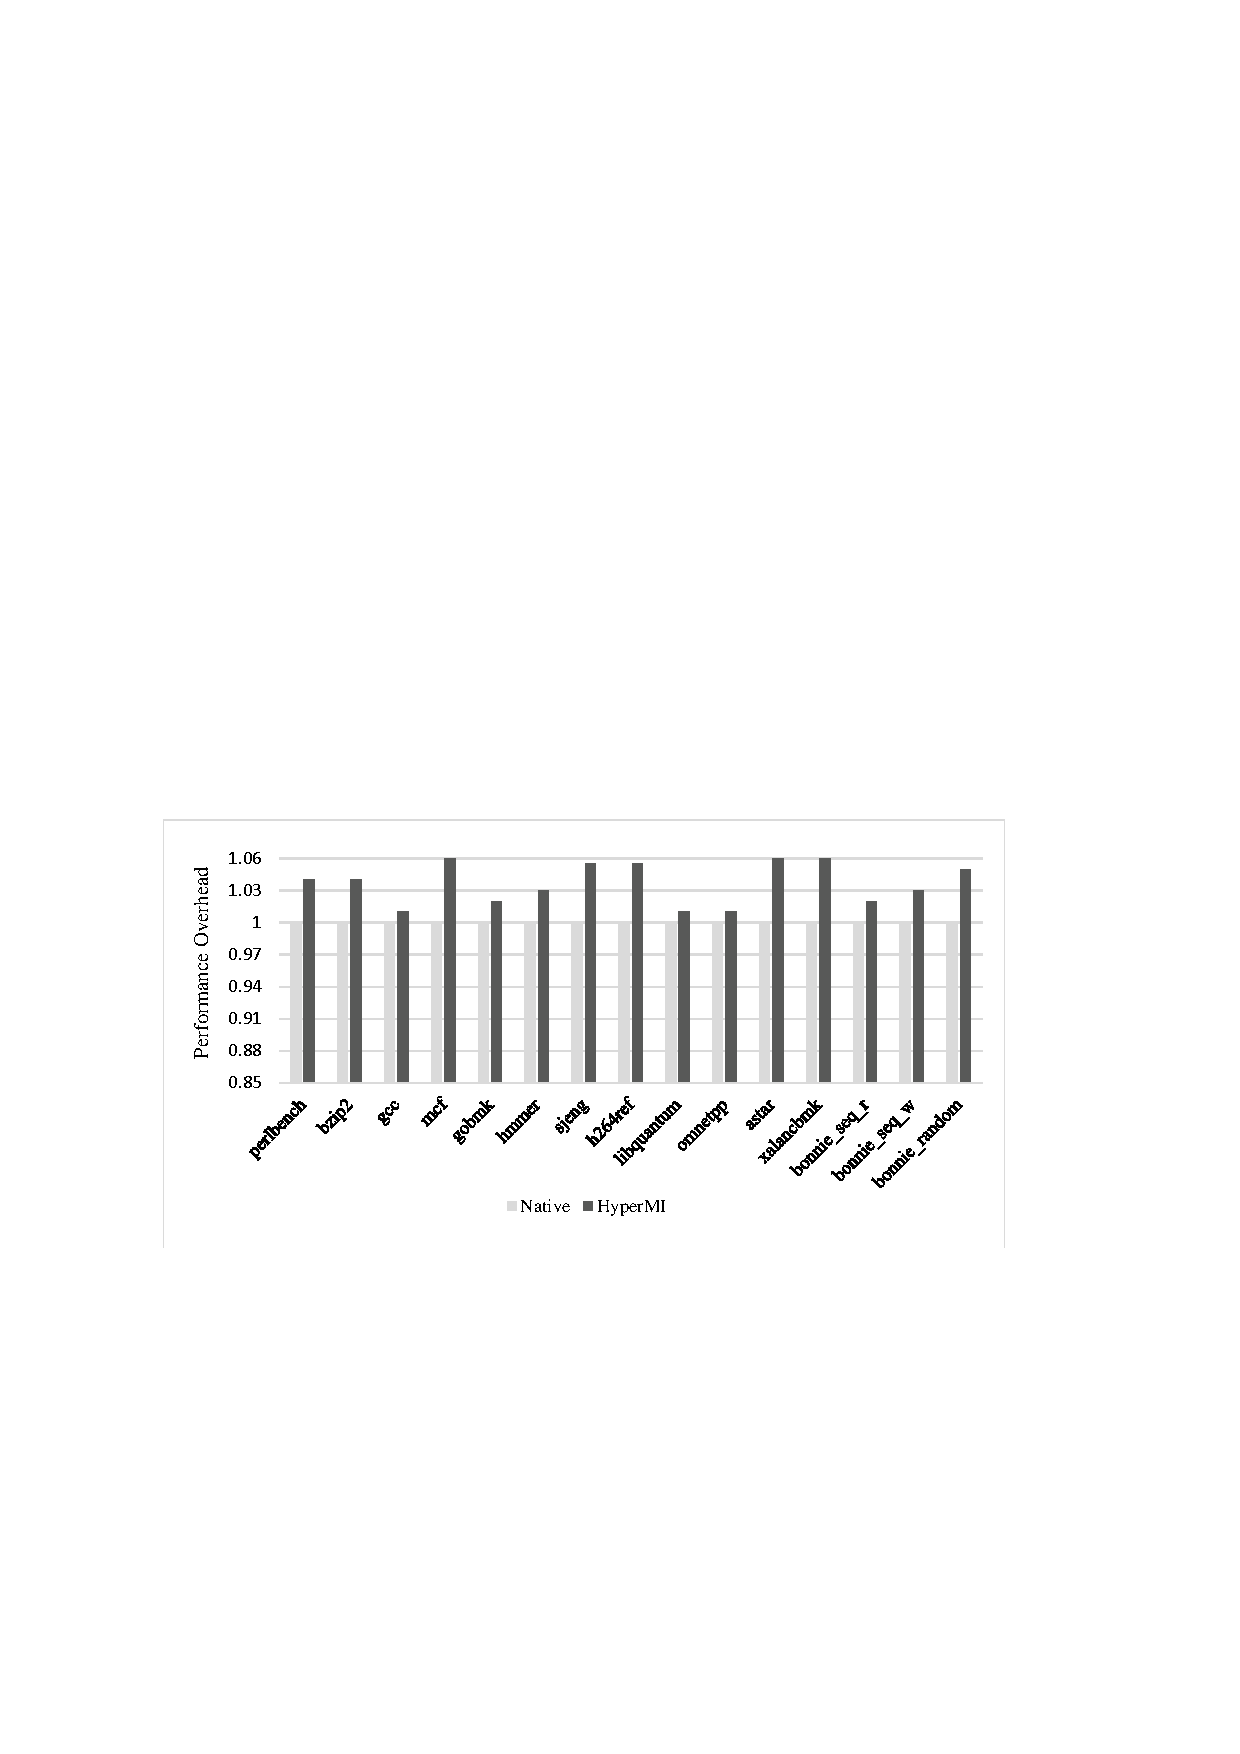
\includegraphics[width=9cm,height=5.5cm]{performance.pdf}}
\caption{Performance overhead.} \label{fig5}
\end{figure}

%\textbf{Macro Benchmarks}
To better understand the factor causing the performance overhead, we experiment with compute-bound benchmark (SPEC CPU2006 suite) and one I/O-bound benchmark (Bonnie++) running upon original KVM and HyperMI in a Linux VM. For Bonnie++, we choose a 1000 MB file to perform the sequential read, write and random access. The experiments result described in Figure \ref{fig5}(the last three groups) shows relatively low cost. Most of the SPEC CPU2006 benchmarks (the first twelve groups) show less than 6\% performance overhead. It's not surprising as there are few OS interactions and these tests are compute-bound. Mcf, astar, and xalancbmk with the highest performance loss allocate lots of memory, and HyperMI handles Page-Mark structure when EPT updates. This can incur worlds switching which involves fewer register access and fewer TLB flushes with PCID technique because the two worlds are at the same privileged layer. For Bonnie++, the performance loss of sequential read, write and random access is 2\%, 3\% and 5\%, the main reason is that HyperMI has no extra memory operations for I/O data. 

\section{Related work}
We describe the related work from these four aspects, integrity verification for hypervisor, reconstructed hypervisor, customized hardware, and the same privilege level isolation. The first aspect is considered from the perspective of protecting the hypervisor, and the other three aspect are considered from the perspective of protecting the VM.

%\subsection{Protection for Hypervisor}

\subsection{Integrity Verification for Hypervisor}
In order to ensure the security of the hypervisor during trusted boot and runtime, an effective and commonly used method is to verify the integrity of the hypervisor, and reduce the attack surface. For the security of the hypervisor during trusted boot, paper \cite{Petroni2007Automated} proposes control flow integrity protection policy, by verifying regularly control flow integrity behavior to detect rootkit attacks. However, attacker can detect the regular and bypass the detection. For runtime security of the hypervisor, HyperSafe \cite{Wang2010HyperSafe} and HyperCheck \cite{Wang2010HyperCheck} choose pooling-query method based on SMM to finish integrity verification of hypervisor. However, SMM doesn't support for MMU. And attackers can hide trace during polling-query intervals when comparing to event-driven monitoring.

%\subsection{Resource Isolation}

\subsection{Customized Hardware }
Some works at the hardware level complete the protection of the process by extending the virtualization capabilities. These tasks provide fine-grained isolation of processes and modules from the hardware level. Haven \cite{haven} uses Intel SGX\cite{Hoekstra13cuvillo,Mckeen2013Innovative} to isolate cloud services from other services and prevent cross-domain access. SGX provides fine-grained protection at the application space instead of hypervisor space, and needs developers spend time reconstructing code and dividing code into trusted part or untrusted part. SGX has requirement for version of CPU. The effort \cite{Cho2016Hardware} combines the advantages of ARM TrustZone and virtualization to improve system performance, and isolate critical process components securely and efficiently. H-SVM\cite{Jin2015H} utilizes the hardware extension features of the CPU, and extends SMM microcode to achieve memory resource isolation among virtual machines. It deprives ability of accessing to memory resource by replacing the source code of the original hypervisor to access memory resource. Vigilare\cite{Moon2012Vigilare} and KI-Mon \cite{Lee2013KI} provide monitoring for access operations by introducing extra hardware. Vigilare provides a kernel integrity monitor that is architected to snoop the bus traffic of the host system from a separate independent hardware. It adds extra Snooper hardware connections module to the host system for bus snooping. KI-Mon monitors write operation to system bus and handles data to write in order to check rootkit attack.
%However, for cloud providers, these approaches means high-cost and low practicality as long as they are carried out widely.
%KI-Mon monitors write operation on system bus and handles data to write in order to check rootkit attack.

\subsection{Reconstructed Hypervisor }
Except for approaches based on hardware, some works\cite{nexen,Steinberg2010NOVA,hyperlock} pay attention to software isolation. Pre-allocating physical resource and completed isolated environment for every VM can avoid VM cross-domain attack, and data leaking attack. NOVA\cite{Steinberg2010NOVA} divides hypervisor into micro-hypervisor and user hypervisor running in root mode, adopts an idea which is similar to fault domain isolation to guarantee an isolated user hypervisor for every VM. The drawback of this approach is the lack of fractional traditional hypervisor functions. HyperLock \cite{hyperlock} prepares backup KVM for every VM by copying KVM code, and ensures every VM run in own isolated space. Nexen\cite{nexen} reconstructs the XEN hypervisor into one privileged security monitor, one component for shared service, backup XEN code and data for every VM, to resist attacker from exploiting known XEN vulnerabilities. These approaches redesign hypervisor greatly. In contrary, HyperMI adopts a feasible way to isolate VM without lots of modification to hypervisor. 

\subsection{The Same Privilege Level Isolation}
Some efforts, ED-Monitor\cite{Deng2017Dancing}, SKEE\cite{Azab2016SKEE} and SecPod\cite{Wang2015SecPod}, adopt the same privilege level idea to avoid performance overhead of inter-level translation. ED-Monitor presents a novel approach that enables practical event-driven monitoring for compromised hypervisor in cloud computing, adopts "the same privilege level" protection against an untrusted hypervisor. The created monitor is placed at the same privilege level and in the same space with hypervisor. SKEE provides a lightweight secure kernel-level execution environment for ARM, this environment is placed at the same privilege level with kernel. When kernel is compromised, attacker can't break the isolation between SKEE and the kernel, and the security of internal security tools placed at secure isolated environment is guaranteed. SecPod, an extensible approach for virtualization-based security systems that can provide both strong isolation and the compatibility with modern hardware. SecPod has two key techniques: paging delegation delegates and audits the kernel's paging operations to a secure space; execution trapping intercepts the (compromised) kernel's attempts to subvert SecPod by misusing privileged instructions.

\section{Conclusion}
We introduce HyperMI, an approach that enables x86 platforms to support a secure isolated execution environment at the same privilege level with hypervisor. The environment is designed to provide memory isolation protection for VM, and secure and event-driven runtime monitoring for interaction between hypervisor and VMs. This approach, which does not rely on additional hardware devices or a higher privilege level software, has fewer changes to system and fewer requirements for types of CPU hardware device. It reflects good practicality and portability. And security analysis describes protection for VM, the performance evaluation shows its efficiency by introducing negligible performance overhead. It can be implemented widely in real-world for cloud providers.


\bibliographystyle{splncs04} 
\bibliography{ref}
\end{document}
